\documentclass[10pt,twocolumn]{article}
\usepackage[a4paper,margin=18mm,columnsep=6mm]{geometry}
\usepackage[T1]{fontenc}
\usepackage{mathptmx}
\usepackage{microtype}
\usepackage{graphicx}
\usepackage{booktabs}
\usepackage[numbers,sort&compress]{natbib}
\usepackage{enumitem}
\usepackage[font=small,labelfont=bf]{caption}
\usepackage[hidelinks]{hyperref}
\setlist{nosep,leftmargin=*}
% Generated by paper/make_numbers.py from the result files. Do not edit by hand.
\makeatletter
\expandafter\def\csname val@bb@all_scored@cnn_ensemble\endcsname{0.741}
\expandafter\def\csname val@bb@all_scored@cnn_ensemble_hi\endcsname{0.785}
\expandafter\def\csname val@bb@all_scored@cnn_ensemble_lo\endcsname{0.683}
\expandafter\def\csname val@bb@all_scored@fusion\endcsname{0.761}
\expandafter\def\csname val@bb@all_scored@fusion_hi\endcsname{0.803}
\expandafter\def\csname val@bb@all_scored@fusion_lo\endcsname{0.703}
\expandafter\def\csname val@bb@all_scored@v2\endcsname{0.661}
\expandafter\def\csname val@bb@all_scored@v2_hi\endcsname{0.720}
\expandafter\def\csname val@bb@all_scored@v2_lo\endcsname{0.600}
\expandafter\def\csname val@bb@paired@cnn_ensemble_minus_bitbrain_vendor_covered\endcsname{-0.041}
\expandafter\def\csname val@bb@paired@cnn_ensemble_minus_bitbrain_vendor_covered_hi\endcsname{-0.015}
\expandafter\def\csname val@bb@paired@cnn_ensemble_minus_bitbrain_vendor_covered_lo\endcsname{-0.069}
\expandafter\def\csname val@bb@paired@fusion_minus_bitbrain_vendor_covered\endcsname{-0.021}
\expandafter\def\csname val@bb@paired@fusion_minus_bitbrain_vendor_covered_hi\endcsname{0.003}
\expandafter\def\csname val@bb@paired@fusion_minus_bitbrain_vendor_covered_lo\endcsname{-0.044}
\expandafter\def\csname val@bb@paired@fusion_minus_cnn_ensemble_all_scored\endcsname{0.020}
\expandafter\def\csname val@bb@paired@fusion_minus_cnn_ensemble_all_scored_hi\endcsname{0.032}
\expandafter\def\csname val@bb@paired@fusion_minus_cnn_ensemble_all_scored_lo\endcsname{0.008}
\expandafter\def\csname val@bb@vendor_covered@bitbrain\endcsname{0.787}
\expandafter\def\csname val@bb@vendor_covered@bitbrain_hi\endcsname{0.826}
\expandafter\def\csname val@bb@vendor_covered@bitbrain_lo\endcsname{0.737}
\expandafter\def\csname val@bb@vendor_covered@cnn_ensemble\endcsname{0.746}
\expandafter\def\csname val@bb@vendor_covered@cnn_ensemble_hi\endcsname{0.790}
\expandafter\def\csname val@bb@vendor_covered@cnn_ensemble_lo\endcsname{0.686}
\expandafter\def\csname val@bb@vendor_covered@fusion\endcsname{0.767}
\expandafter\def\csname val@bb@vendor_covered@fusion_hi\endcsname{0.809}
\expandafter\def\csname val@bb@vendor_covered@fusion_lo\endcsname{0.708}
\expandafter\def\csname val@bb@vendor_covered@v2\endcsname{0.666}
\expandafter\def\csname val@bb@vendor_covered@v2_hi\endcsname{0.723}
\expandafter\def\csname val@bb@vendor_covered@v2_lo\endcsname{0.605}
\expandafter\def\csname val@bb@w@v2\endcsname{0.3}
\expandafter\def\csname val@boas@cnn@kappa\endcsname{0.728}
\expandafter\def\csname val@boas@cnn@kappa_hi\endcsname{0.772}
\expandafter\def\csname val@boas@cnn@kappa_lo\endcsname{0.670}
\expandafter\def\csname val@boas@cnn@macro_f1\endcsname{0.595}
\expandafter\def\csname val@boas@cnn@macro_f1_hi\endcsname{0.636}
\expandafter\def\csname val@boas@cnn@macro_f1_lo\endcsname{0.553}
\expandafter\def\csname val@boas@cnn@tst_error_minutes\endcsname{16.5}
\expandafter\def\csname val@boas@cnn@tst_error_minutes_hi\endcsname{25.9}
\expandafter\def\csname val@boas@cnn@tst_error_minutes_lo\endcsname{8.3}
\expandafter\def\csname val@boas@cnn@wake_f1\endcsname{0.812}
\expandafter\def\csname val@boas@cnn@wake_f1_hi\endcsname{0.859}
\expandafter\def\csname val@boas@cnn@wake_f1_lo\endcsname{0.761}
\expandafter\def\csname val@boas@cnn@wake_recall\endcsname{0.868}
\expandafter\def\csname val@boas@cnn@wake_recall_hi\endcsname{0.909}
\expandafter\def\csname val@boas@cnn@wake_recall_lo\endcsname{0.821}
\expandafter\def\csname val@boas@cnn_augmented@kappa\endcsname{0.727}
\expandafter\def\csname val@boas@cnn_augmented@kappa_hi\endcsname{0.772}
\expandafter\def\csname val@boas@cnn_augmented@kappa_lo\endcsname{0.663}
\expandafter\def\csname val@boas@cnn_augmented@macro_f1\endcsname{0.591}
\expandafter\def\csname val@boas@cnn_augmented@macro_f1_hi\endcsname{0.631}
\expandafter\def\csname val@boas@cnn_augmented@macro_f1_lo\endcsname{0.550}
\expandafter\def\csname val@boas@cnn_augmented@tst_error_minutes\endcsname{11.5}
\expandafter\def\csname val@boas@cnn_augmented@tst_error_minutes_hi\endcsname{18.5}
\expandafter\def\csname val@boas@cnn_augmented@tst_error_minutes_lo\endcsname{6.0}
\expandafter\def\csname val@boas@cnn_augmented@wake_f1\endcsname{0.830}
\expandafter\def\csname val@boas@cnn_augmented@wake_f1_hi\endcsname{0.870}
\expandafter\def\csname val@boas@cnn_augmented@wake_f1_lo\endcsname{0.781}
\expandafter\def\csname val@boas@cnn_augmented@wake_recall\endcsname{0.846}
\expandafter\def\csname val@boas@cnn_augmented@wake_recall_hi\endcsname{0.893}
\expandafter\def\csname val@boas@cnn_augmented@wake_recall_lo\endcsname{0.794}
\expandafter\def\csname val@boas@cnn_balanced@kappa\endcsname{0.479}
\expandafter\def\csname val@boas@cnn_balanced@kappa_hi\endcsname{0.535}
\expandafter\def\csname val@boas@cnn_balanced@kappa_lo\endcsname{0.421}
\expandafter\def\csname val@boas@cnn_balanced@macro_f1\endcsname{0.525}
\expandafter\def\csname val@boas@cnn_balanced@macro_f1_hi\endcsname{0.569}
\expandafter\def\csname val@boas@cnn_balanced@macro_f1_lo\endcsname{0.478}
\expandafter\def\csname val@boas@cnn_balanced@tst_error_minutes\endcsname{8.4}
\expandafter\def\csname val@boas@cnn_balanced@tst_error_minutes_hi\endcsname{11.8}
\expandafter\def\csname val@boas@cnn_balanced@tst_error_minutes_lo\endcsname{5.3}
\expandafter\def\csname val@boas@cnn_balanced@wake_f1\endcsname{0.770}
\expandafter\def\csname val@boas@cnn_balanced@wake_f1_hi\endcsname{0.820}
\expandafter\def\csname val@boas@cnn_balanced@wake_f1_lo\endcsname{0.717}
\expandafter\def\csname val@boas@cnn_balanced@wake_recall\endcsname{0.734}
\expandafter\def\csname val@boas@cnn_balanced@wake_recall_hi\endcsname{0.803}
\expandafter\def\csname val@boas@cnn_balanced@wake_recall_lo\endcsname{0.663}
\expandafter\def\csname val@boas@cnn_context@kappa\endcsname{0.734}
\expandafter\def\csname val@boas@cnn_context@kappa_hi\endcsname{0.779}
\expandafter\def\csname val@boas@cnn_context@kappa_lo\endcsname{0.676}
\expandafter\def\csname val@boas@cnn_context@macro_f1\endcsname{0.618}
\expandafter\def\csname val@boas@cnn_context@macro_f1_hi\endcsname{0.661}
\expandafter\def\csname val@boas@cnn_context@macro_f1_lo\endcsname{0.575}
\expandafter\def\csname val@boas@cnn_context@tst_error_minutes\endcsname{8.7}
\expandafter\def\csname val@boas@cnn_context@tst_error_minutes_hi\endcsname{12.2}
\expandafter\def\csname val@boas@cnn_context@tst_error_minutes_lo\endcsname{5.5}
\expandafter\def\csname val@boas@cnn_context@wake_f1\endcsname{0.817}
\expandafter\def\csname val@boas@cnn_context@wake_f1_hi\endcsname{0.870}
\expandafter\def\csname val@boas@cnn_context@wake_f1_lo\endcsname{0.757}
\expandafter\def\csname val@boas@cnn_context@wake_recall\endcsname{0.815}
\expandafter\def\csname val@boas@cnn_context@wake_recall_hi\endcsname{0.872}
\expandafter\def\csname val@boas@cnn_context@wake_recall_lo\endcsname{0.751}
\expandafter\def\csname val@boas@cnn_context_balanced@kappa\endcsname{0.712}
\expandafter\def\csname val@boas@cnn_context_balanced@kappa_hi\endcsname{0.755}
\expandafter\def\csname val@boas@cnn_context_balanced@kappa_lo\endcsname{0.657}
\expandafter\def\csname val@boas@cnn_context_balanced@macro_f1\endcsname{0.592}
\expandafter\def\csname val@boas@cnn_context_balanced@macro_f1_hi\endcsname{0.631}
\expandafter\def\csname val@boas@cnn_context_balanced@macro_f1_lo\endcsname{0.552}
\expandafter\def\csname val@boas@cnn_context_balanced@tst_error_minutes\endcsname{10.1}
\expandafter\def\csname val@boas@cnn_context_balanced@tst_error_minutes_hi\endcsname{12.6}
\expandafter\def\csname val@boas@cnn_context_balanced@tst_error_minutes_lo\endcsname{7.8}
\expandafter\def\csname val@boas@cnn_context_balanced@wake_f1\endcsname{0.793}
\expandafter\def\csname val@boas@cnn_context_balanced@wake_f1_hi\endcsname{0.853}
\expandafter\def\csname val@boas@cnn_context_balanced@wake_f1_lo\endcsname{0.725}
\expandafter\def\csname val@boas@cnn_context_balanced@wake_recall\endcsname{0.748}
\expandafter\def\csname val@boas@cnn_context_balanced@wake_recall_hi\endcsname{0.827}
\expandafter\def\csname val@boas@cnn_context_balanced@wake_recall_lo\endcsname{0.659}
\expandafter\def\csname val@boas@cnn_context_sqrtbalanced@kappa\endcsname{0.737}
\expandafter\def\csname val@boas@cnn_context_sqrtbalanced@kappa_hi\endcsname{0.782}
\expandafter\def\csname val@boas@cnn_context_sqrtbalanced@kappa_lo\endcsname{0.679}
\expandafter\def\csname val@boas@cnn_context_sqrtbalanced@macro_f1\endcsname{0.607}
\expandafter\def\csname val@boas@cnn_context_sqrtbalanced@macro_f1_hi\endcsname{0.645}
\expandafter\def\csname val@boas@cnn_context_sqrtbalanced@macro_f1_lo\endcsname{0.567}
\expandafter\def\csname val@boas@cnn_context_sqrtbalanced@tst_error_minutes\endcsname{10.2}
\expandafter\def\csname val@boas@cnn_context_sqrtbalanced@tst_error_minutes_hi\endcsname{14.6}
\expandafter\def\csname val@boas@cnn_context_sqrtbalanced@tst_error_minutes_lo\endcsname{6.4}
\expandafter\def\csname val@boas@cnn_context_sqrtbalanced@wake_f1\endcsname{0.813}
\expandafter\def\csname val@boas@cnn_context_sqrtbalanced@wake_f1_hi\endcsname{0.863}
\expandafter\def\csname val@boas@cnn_context_sqrtbalanced@wake_f1_lo\endcsname{0.757}
\expandafter\def\csname val@boas@cnn_context_sqrtbalanced@wake_recall\endcsname{0.817}
\expandafter\def\csname val@boas@cnn_context_sqrtbalanced@wake_recall_hi\endcsname{0.875}
\expandafter\def\csname val@boas@cnn_context_sqrtbalanced@wake_recall_lo\endcsname{0.750}
\expandafter\def\csname val@boas@cnn_sqrtbalanced@kappa\endcsname{0.662}
\expandafter\def\csname val@boas@cnn_sqrtbalanced@kappa_hi\endcsname{0.713}
\expandafter\def\csname val@boas@cnn_sqrtbalanced@kappa_lo\endcsname{0.600}
\expandafter\def\csname val@boas@cnn_sqrtbalanced@macro_f1\endcsname{0.604}
\expandafter\def\csname val@boas@cnn_sqrtbalanced@macro_f1_hi\endcsname{0.649}
\expandafter\def\csname val@boas@cnn_sqrtbalanced@macro_f1_lo\endcsname{0.555}
\expandafter\def\csname val@boas@cnn_sqrtbalanced@tst_error_minutes\endcsname{9.8}
\expandafter\def\csname val@boas@cnn_sqrtbalanced@tst_error_minutes_hi\endcsname{12.8}
\expandafter\def\csname val@boas@cnn_sqrtbalanced@tst_error_minutes_lo\endcsname{7.0}
\expandafter\def\csname val@boas@cnn_sqrtbalanced@wake_f1\endcsname{0.795}
\expandafter\def\csname val@boas@cnn_sqrtbalanced@wake_f1_hi\endcsname{0.844}
\expandafter\def\csname val@boas@cnn_sqrtbalanced@wake_f1_lo\endcsname{0.739}
\expandafter\def\csname val@boas@cnn_sqrtbalanced@wake_recall\endcsname{0.738}
\expandafter\def\csname val@boas@cnn_sqrtbalanced@wake_recall_hi\endcsname{0.801}
\expandafter\def\csname val@boas@cnn_sqrtbalanced@wake_recall_lo\endcsname{0.670}
\expandafter\def\csname val@boas@v2@kappa\endcsname{0.661}
\expandafter\def\csname val@boas@v2@kappa_hi\endcsname{0.717}
\expandafter\def\csname val@boas@v2@kappa_lo\endcsname{0.598}
\expandafter\def\csname val@boas@v2@macro_f1\endcsname{0.561}
\expandafter\def\csname val@boas@v2@macro_f1_hi\endcsname{0.606}
\expandafter\def\csname val@boas@v2@macro_f1_lo\endcsname{0.514}
\expandafter\def\csname val@boas@v2@tst_error_minutes\endcsname{31.8}
\expandafter\def\csname val@boas@v2@tst_error_minutes_hi\endcsname{50.2}
\expandafter\def\csname val@boas@v2@tst_error_minutes_lo\endcsname{16.7}
\expandafter\def\csname val@boas@v2@wake_f1\endcsname{0.767}
\expandafter\def\csname val@boas@v2@wake_f1_hi\endcsname{0.827}
\expandafter\def\csname val@boas@v2@wake_f1_lo\endcsname{0.702}
\expandafter\def\csname val@boas@v2@wake_recall\endcsname{0.858}
\expandafter\def\csname val@boas@v2@wake_recall_hi\endcsname{0.923}
\expandafter\def\csname val@boas@v2@wake_recall_lo\endcsname{0.775}
\expandafter\def\csname val@boas@yasa@kappa\endcsname{0.532}
\expandafter\def\csname val@boas@yasa@kappa_hi\endcsname{0.590}
\expandafter\def\csname val@boas@yasa@kappa_lo\endcsname{0.470}
\expandafter\def\csname val@boas@yasa@macro_f1\endcsname{0.518}
\expandafter\def\csname val@boas@yasa@macro_f1_hi\endcsname{0.565}
\expandafter\def\csname val@boas@yasa@macro_f1_lo\endcsname{0.471}
\expandafter\def\csname val@boas@yasa@tst_error_minutes\endcsname{57.6}
\expandafter\def\csname val@boas@yasa@tst_error_minutes_hi\endcsname{81.9}
\expandafter\def\csname val@boas@yasa@tst_error_minutes_lo\endcsname{35.6}
\expandafter\def\csname val@boas@yasa@wake_f1\endcsname{0.704}
\expandafter\def\csname val@boas@yasa@wake_f1_hi\endcsname{0.770}
\expandafter\def\csname val@boas@yasa@wake_f1_lo\endcsname{0.640}
\expandafter\def\csname val@boas@yasa@wake_recall\endcsname{0.976}
\expandafter\def\csname val@boas@yasa@wake_recall_hi\endcsname{0.991}
\expandafter\def\csname val@boas@yasa@wake_recall_lo\endcsname{0.955}
\expandafter\def\csname val@dodh@cnn@kappa\endcsname{0.297}
\expandafter\def\csname val@dodh@cnn@kappa_hi\endcsname{0.357}
\expandafter\def\csname val@dodh@cnn@kappa_lo\endcsname{0.238}
\expandafter\def\csname val@dodh@cnn@macro_f1\endcsname{0.363}
\expandafter\def\csname val@dodh@cnn@macro_f1_hi\endcsname{0.402}
\expandafter\def\csname val@dodh@cnn@macro_f1_lo\endcsname{0.328}
\expandafter\def\csname val@dodh@cnn@tst_error_minutes\endcsname{26.8}
\expandafter\def\csname val@dodh@cnn@tst_error_minutes_hi\endcsname{36.5}
\expandafter\def\csname val@dodh@cnn@tst_error_minutes_lo\endcsname{18.2}
\expandafter\def\csname val@dodh@cnn@wake_f1\endcsname{0.536}
\expandafter\def\csname val@dodh@cnn@wake_f1_hi\endcsname{0.616}
\expandafter\def\csname val@dodh@cnn@wake_f1_lo\endcsname{0.452}
\expandafter\def\csname val@dodh@cnn@wake_recall\endcsname{0.503}
\expandafter\def\csname val@dodh@cnn@wake_recall_hi\endcsname{0.586}
\expandafter\def\csname val@dodh@cnn@wake_recall_lo\endcsname{0.422}
\expandafter\def\csname val@dodh@cnn_augmented@kappa\endcsname{0.331}
\expandafter\def\csname val@dodh@cnn_augmented@kappa_hi\endcsname{0.391}
\expandafter\def\csname val@dodh@cnn_augmented@kappa_lo\endcsname{0.276}
\expandafter\def\csname val@dodh@cnn_augmented@macro_f1\endcsname{0.383}
\expandafter\def\csname val@dodh@cnn_augmented@macro_f1_hi\endcsname{0.422}
\expandafter\def\csname val@dodh@cnn_augmented@macro_f1_lo\endcsname{0.347}
\expandafter\def\csname val@dodh@cnn_augmented@tst_error_minutes\endcsname{27.9}
\expandafter\def\csname val@dodh@cnn_augmented@tst_error_minutes_hi\endcsname{37.3}
\expandafter\def\csname val@dodh@cnn_augmented@tst_error_minutes_lo\endcsname{19.3}
\expandafter\def\csname val@dodh@cnn_augmented@wake_f1\endcsname{0.516}
\expandafter\def\csname val@dodh@cnn_augmented@wake_f1_hi\endcsname{0.602}
\expandafter\def\csname val@dodh@cnn_augmented@wake_f1_lo\endcsname{0.430}
\expandafter\def\csname val@dodh@cnn_augmented@wake_recall\endcsname{0.473}
\expandafter\def\csname val@dodh@cnn_augmented@wake_recall_hi\endcsname{0.559}
\expandafter\def\csname val@dodh@cnn_augmented@wake_recall_lo\endcsname{0.386}
\expandafter\def\csname val@dodh@cnn_balanced@kappa\endcsname{0.445}
\expandafter\def\csname val@dodh@cnn_balanced@kappa_hi\endcsname{0.503}
\expandafter\def\csname val@dodh@cnn_balanced@kappa_lo\endcsname{0.384}
\expandafter\def\csname val@dodh@cnn_balanced@macro_f1\endcsname{0.517}
\expandafter\def\csname val@dodh@cnn_balanced@macro_f1_hi\endcsname{0.561}
\expandafter\def\csname val@dodh@cnn_balanced@macro_f1_lo\endcsname{0.469}
\expandafter\def\csname val@dodh@cnn_balanced@tst_error_minutes\endcsname{28.7}
\expandafter\def\csname val@dodh@cnn_balanced@tst_error_minutes_hi\endcsname{43.0}
\expandafter\def\csname val@dodh@cnn_balanced@tst_error_minutes_lo\endcsname{17.5}
\expandafter\def\csname val@dodh@cnn_balanced@wake_f1\endcsname{0.511}
\expandafter\def\csname val@dodh@cnn_balanced@wake_f1_hi\endcsname{0.586}
\expandafter\def\csname val@dodh@cnn_balanced@wake_f1_lo\endcsname{0.433}
\expandafter\def\csname val@dodh@cnn_balanced@wake_recall\endcsname{0.519}
\expandafter\def\csname val@dodh@cnn_balanced@wake_recall_hi\endcsname{0.594}
\expandafter\def\csname val@dodh@cnn_balanced@wake_recall_lo\endcsname{0.444}
\expandafter\def\csname val@dodh@cnn_context@kappa\endcsname{0.325}
\expandafter\def\csname val@dodh@cnn_context@kappa_hi\endcsname{0.391}
\expandafter\def\csname val@dodh@cnn_context@kappa_lo\endcsname{0.258}
\expandafter\def\csname val@dodh@cnn_context@macro_f1\endcsname{0.414}
\expandafter\def\csname val@dodh@cnn_context@macro_f1_hi\endcsname{0.461}
\expandafter\def\csname val@dodh@cnn_context@macro_f1_lo\endcsname{0.369}
\expandafter\def\csname val@dodh@cnn_context@tst_error_minutes\endcsname{35.1}
\expandafter\def\csname val@dodh@cnn_context@tst_error_minutes_hi\endcsname{45.9}
\expandafter\def\csname val@dodh@cnn_context@tst_error_minutes_lo\endcsname{26.4}
\expandafter\def\csname val@dodh@cnn_context@wake_f1\endcsname{0.418}
\expandafter\def\csname val@dodh@cnn_context@wake_f1_hi\endcsname{0.503}
\expandafter\def\csname val@dodh@cnn_context@wake_f1_lo\endcsname{0.333}
\expandafter\def\csname val@dodh@cnn_context@wake_recall\endcsname{0.332}
\expandafter\def\csname val@dodh@cnn_context@wake_recall_hi\endcsname{0.414}
\expandafter\def\csname val@dodh@cnn_context@wake_recall_lo\endcsname{0.255}
\expandafter\def\csname val@dodh@cnn_context_balanced@kappa\endcsname{0.221}
\expandafter\def\csname val@dodh@cnn_context_balanced@kappa_hi\endcsname{0.285}
\expandafter\def\csname val@dodh@cnn_context_balanced@kappa_lo\endcsname{0.159}
\expandafter\def\csname val@dodh@cnn_context_balanced@macro_f1\endcsname{0.327}
\expandafter\def\csname val@dodh@cnn_context_balanced@macro_f1_hi\endcsname{0.371}
\expandafter\def\csname val@dodh@cnn_context_balanced@macro_f1_lo\endcsname{0.284}
\expandafter\def\csname val@dodh@cnn_context_balanced@tst_error_minutes\endcsname{45.1}
\expandafter\def\csname val@dodh@cnn_context_balanced@tst_error_minutes_hi\endcsname{57.1}
\expandafter\def\csname val@dodh@cnn_context_balanced@tst_error_minutes_lo\endcsname{34.3}
\expandafter\def\csname val@dodh@cnn_context_balanced@wake_f1\endcsname{0.311}
\expandafter\def\csname val@dodh@cnn_context_balanced@wake_f1_hi\endcsname{0.390}
\expandafter\def\csname val@dodh@cnn_context_balanced@wake_f1_lo\endcsname{0.234}
\expandafter\def\csname val@dodh@cnn_context_balanced@wake_recall\endcsname{0.224}
\expandafter\def\csname val@dodh@cnn_context_balanced@wake_recall_hi\endcsname{0.301}
\expandafter\def\csname val@dodh@cnn_context_balanced@wake_recall_lo\endcsname{0.156}
\expandafter\def\csname val@dodh@cnn_context_sqrtbalanced@kappa\endcsname{0.300}
\expandafter\def\csname val@dodh@cnn_context_sqrtbalanced@kappa_hi\endcsname{0.375}
\expandafter\def\csname val@dodh@cnn_context_sqrtbalanced@kappa_lo\endcsname{0.222}
\expandafter\def\csname val@dodh@cnn_context_sqrtbalanced@macro_f1\endcsname{0.392}
\expandafter\def\csname val@dodh@cnn_context_sqrtbalanced@macro_f1_hi\endcsname{0.444}
\expandafter\def\csname val@dodh@cnn_context_sqrtbalanced@macro_f1_lo\endcsname{0.341}
\expandafter\def\csname val@dodh@cnn_context_sqrtbalanced@tst_error_minutes\endcsname{35.6}
\expandafter\def\csname val@dodh@cnn_context_sqrtbalanced@tst_error_minutes_hi\endcsname{44.9}
\expandafter\def\csname val@dodh@cnn_context_sqrtbalanced@tst_error_minutes_lo\endcsname{27.5}
\expandafter\def\csname val@dodh@cnn_context_sqrtbalanced@wake_f1\endcsname{0.401}
\expandafter\def\csname val@dodh@cnn_context_sqrtbalanced@wake_f1_hi\endcsname{0.485}
\expandafter\def\csname val@dodh@cnn_context_sqrtbalanced@wake_f1_lo\endcsname{0.320}
\expandafter\def\csname val@dodh@cnn_context_sqrtbalanced@wake_recall\endcsname{0.312}
\expandafter\def\csname val@dodh@cnn_context_sqrtbalanced@wake_recall_hi\endcsname{0.397}
\expandafter\def\csname val@dodh@cnn_context_sqrtbalanced@wake_recall_lo\endcsname{0.234}
\expandafter\def\csname val@dodh@cnn_sqrtbalanced@kappa\endcsname{0.393}
\expandafter\def\csname val@dodh@cnn_sqrtbalanced@kappa_hi\endcsname{0.467}
\expandafter\def\csname val@dodh@cnn_sqrtbalanced@kappa_lo\endcsname{0.317}
\expandafter\def\csname val@dodh@cnn_sqrtbalanced@macro_f1\endcsname{0.454}
\expandafter\def\csname val@dodh@cnn_sqrtbalanced@macro_f1_hi\endcsname{0.503}
\expandafter\def\csname val@dodh@cnn_sqrtbalanced@macro_f1_lo\endcsname{0.405}
\expandafter\def\csname val@dodh@cnn_sqrtbalanced@tst_error_minutes\endcsname{34.3}
\expandafter\def\csname val@dodh@cnn_sqrtbalanced@tst_error_minutes_hi\endcsname{43.1}
\expandafter\def\csname val@dodh@cnn_sqrtbalanced@tst_error_minutes_lo\endcsname{26.2}
\expandafter\def\csname val@dodh@cnn_sqrtbalanced@wake_f1\endcsname{0.448}
\expandafter\def\csname val@dodh@cnn_sqrtbalanced@wake_f1_hi\endcsname{0.531}
\expandafter\def\csname val@dodh@cnn_sqrtbalanced@wake_f1_lo\endcsname{0.365}
\expandafter\def\csname val@dodh@cnn_sqrtbalanced@wake_recall\endcsname{0.367}
\expandafter\def\csname val@dodh@cnn_sqrtbalanced@wake_recall_hi\endcsname{0.447}
\expandafter\def\csname val@dodh@cnn_sqrtbalanced@wake_recall_lo\endcsname{0.291}
\expandafter\def\csname val@dodh@ensemble_of_7@kappa\endcsname{0.334}
\expandafter\def\csname val@dodh@ensemble_of_7@kappa_hi\endcsname{0.410}
\expandafter\def\csname val@dodh@ensemble_of_7@kappa_lo\endcsname{0.260}
\expandafter\def\csname val@dodh@ensemble_of_7@macro_f1\endcsname{0.407}
\expandafter\def\csname val@dodh@ensemble_of_7@macro_f1_hi\endcsname{0.459}
\expandafter\def\csname val@dodh@ensemble_of_7@macro_f1_lo\endcsname{0.358}
\expandafter\def\csname val@dodh@ensemble_of_7@tst_error_minutes\endcsname{30.6}
\expandafter\def\csname val@dodh@ensemble_of_7@tst_error_minutes_hi\endcsname{38.4}
\expandafter\def\csname val@dodh@ensemble_of_7@tst_error_minutes_lo\endcsname{23.4}
\expandafter\def\csname val@dodh@ensemble_of_7@wake_f1\endcsname{0.477}
\expandafter\def\csname val@dodh@ensemble_of_7@wake_f1_hi\endcsname{0.563}
\expandafter\def\csname val@dodh@ensemble_of_7@wake_f1_lo\endcsname{0.389}
\expandafter\def\csname val@dodh@ensemble_of_7@wake_recall\endcsname{0.397}
\expandafter\def\csname val@dodh@ensemble_of_7@wake_recall_hi\endcsname{0.485}
\expandafter\def\csname val@dodh@ensemble_of_7@wake_recall_lo\endcsname{0.310}
\expandafter\def\csname val@dodh@v2@kappa\endcsname{0.111}
\expandafter\def\csname val@dodh@v2@kappa_hi\endcsname{0.154}
\expandafter\def\csname val@dodh@v2@kappa_lo\endcsname{0.071}
\expandafter\def\csname val@dodh@v2@macro_f1\endcsname{0.215}
\expandafter\def\csname val@dodh@v2@macro_f1_hi\endcsname{0.240}
\expandafter\def\csname val@dodh@v2@macro_f1_lo\endcsname{0.190}
\expandafter\def\csname val@dodh@v2@tst_error_minutes\endcsname{57.5}
\expandafter\def\csname val@dodh@v2@tst_error_minutes_hi\endcsname{74.7}
\expandafter\def\csname val@dodh@v2@tst_error_minutes_lo\endcsname{42.7}
\expandafter\def\csname val@dodh@v2@wake_f1\endcsname{0.172}
\expandafter\def\csname val@dodh@v2@wake_f1_hi\endcsname{0.260}
\expandafter\def\csname val@dodh@v2@wake_f1_lo\endcsname{0.094}
\expandafter\def\csname val@dodh@v2@wake_recall\endcsname{0.142}
\expandafter\def\csname val@dodh@v2@wake_recall_hi\endcsname{0.230}
\expandafter\def\csname val@dodh@v2@wake_recall_lo\endcsname{0.069}
\expandafter\def\csname val@dodh@v2_gain_q75@kappa\endcsname{0.318}
\expandafter\def\csname val@dodh@v2_gain_q75@kappa_hi\endcsname{0.396}
\expandafter\def\csname val@dodh@v2_gain_q75@kappa_lo\endcsname{0.243}
\expandafter\def\csname val@dodh@v2_gain_q75@macro_f1\endcsname{0.375}
\expandafter\def\csname val@dodh@v2_gain_q75@macro_f1_hi\endcsname{0.425}
\expandafter\def\csname val@dodh@v2_gain_q75@macro_f1_lo\endcsname{0.328}
\expandafter\def\csname val@dodh@v2_gain_q75@tst_error_minutes\endcsname{46.2}
\expandafter\def\csname val@dodh@v2_gain_q75@tst_error_minutes_hi\endcsname{69.3}
\expandafter\def\csname val@dodh@v2_gain_q75@tst_error_minutes_lo\endcsname{28.3}
\expandafter\def\csname val@dodh@v2_gain_q75@wake_f1\endcsname{0.396}
\expandafter\def\csname val@dodh@v2_gain_q75@wake_f1_hi\endcsname{0.503}
\expandafter\def\csname val@dodh@v2_gain_q75@wake_f1_lo\endcsname{0.295}
\expandafter\def\csname val@dodh@v2_gain_q75@wake_recall\endcsname{0.349}
\expandafter\def\csname val@dodh@v2_gain_q75@wake_recall_hi\endcsname{0.464}
\expandafter\def\csname val@dodh@v2_gain_q75@wake_recall_lo\endcsname{0.242}
\expandafter\def\csname val@dodh@v2_gain_q90@kappa\endcsname{0.333}
\expandafter\def\csname val@dodh@v2_gain_q90@kappa_hi\endcsname{0.402}
\expandafter\def\csname val@dodh@v2_gain_q90@kappa_lo\endcsname{0.265}
\expandafter\def\csname val@dodh@v2_gain_q90@macro_f1\endcsname{0.388}
\expandafter\def\csname val@dodh@v2_gain_q90@macro_f1_hi\endcsname{0.433}
\expandafter\def\csname val@dodh@v2_gain_q90@macro_f1_lo\endcsname{0.344}
\expandafter\def\csname val@dodh@v2_gain_q90@tst_error_minutes\endcsname{44.5}
\expandafter\def\csname val@dodh@v2_gain_q90@tst_error_minutes_hi\endcsname{68.7}
\expandafter\def\csname val@dodh@v2_gain_q90@tst_error_minutes_lo\endcsname{26.9}
\expandafter\def\csname val@dodh@v2_gain_q90@wake_f1\endcsname{0.471}
\expandafter\def\csname val@dodh@v2_gain_q90@wake_f1_hi\endcsname{0.569}
\expandafter\def\csname val@dodh@v2_gain_q90@wake_f1_lo\endcsname{0.371}
\expandafter\def\csname val@dodh@v2_gain_q90@wake_recall\endcsname{0.453}
\expandafter\def\csname val@dodh@v2_gain_q90@wake_recall_hi\endcsname{0.565}
\expandafter\def\csname val@dodh@v2_gain_q90@wake_recall_lo\endcsname{0.344}
\expandafter\def\csname val@dodh@yasa@kappa\endcsname{0.655}
\expandafter\def\csname val@dodh@yasa@kappa_hi\endcsname{0.719}
\expandafter\def\csname val@dodh@yasa@kappa_lo\endcsname{0.584}
\expandafter\def\csname val@dodh@yasa@macro_f1\endcsname{0.654}
\expandafter\def\csname val@dodh@yasa@macro_f1_hi\endcsname{0.704}
\expandafter\def\csname val@dodh@yasa@macro_f1_lo\endcsname{0.599}
\expandafter\def\csname val@dodh@yasa@tst_error_minutes\endcsname{23.4}
\expandafter\def\csname val@dodh@yasa@tst_error_minutes_hi\endcsname{45.2}
\expandafter\def\csname val@dodh@yasa@tst_error_minutes_lo\endcsname{9.4}
\expandafter\def\csname val@dodh@yasa@wake_f1\endcsname{0.663}
\expandafter\def\csname val@dodh@yasa@wake_f1_hi\endcsname{0.741}
\expandafter\def\csname val@dodh@yasa@wake_f1_lo\endcsname{0.578}
\expandafter\def\csname val@dodh@yasa@wake_recall\endcsname{0.703}
\expandafter\def\csname val@dodh@yasa@wake_recall_hi\endcsname{0.772}
\expandafter\def\csname val@dodh@yasa@wake_recall_lo\endcsname{0.629}
\expandafter\def\csname val@gain@dodh@q75\endcsname{4.06}
\expandafter\def\csname val@gain@hmc@q75\endcsname{1.38}
\expandafter\def\csname val@hmc@cnn@kappa\endcsname{0.372}
\expandafter\def\csname val@hmc@cnn@kappa_hi\endcsname{0.413}
\expandafter\def\csname val@hmc@cnn@kappa_lo\endcsname{0.329}
\expandafter\def\csname val@hmc@cnn@macro_f1\endcsname{0.421}
\expandafter\def\csname val@hmc@cnn@macro_f1_hi\endcsname{0.449}
\expandafter\def\csname val@hmc@cnn@macro_f1_lo\endcsname{0.388}
\expandafter\def\csname val@hmc@cnn@tst_error_minutes\endcsname{21.7}
\expandafter\def\csname val@hmc@cnn@tst_error_minutes_hi\endcsname{38.1}
\expandafter\def\csname val@hmc@cnn@tst_error_minutes_lo\endcsname{10.3}
\expandafter\def\csname val@hmc@cnn@wake_f1\endcsname{0.605}
\expandafter\def\csname val@hmc@cnn@wake_f1_hi\endcsname{0.672}
\expandafter\def\csname val@hmc@cnn@wake_f1_lo\endcsname{0.533}
\expandafter\def\csname val@hmc@cnn@wake_recall\endcsname{0.638}
\expandafter\def\csname val@hmc@cnn@wake_recall_hi\endcsname{0.709}
\expandafter\def\csname val@hmc@cnn@wake_recall_lo\endcsname{0.560}
\expandafter\def\csname val@hmc@cnn_augmented@kappa\endcsname{0.375}
\expandafter\def\csname val@hmc@cnn_augmented@kappa_hi\endcsname{0.417}
\expandafter\def\csname val@hmc@cnn_augmented@kappa_lo\endcsname{0.330}
\expandafter\def\csname val@hmc@cnn_augmented@macro_f1\endcsname{0.420}
\expandafter\def\csname val@hmc@cnn_augmented@macro_f1_hi\endcsname{0.451}
\expandafter\def\csname val@hmc@cnn_augmented@macro_f1_lo\endcsname{0.386}
\expandafter\def\csname val@hmc@cnn_augmented@tst_error_minutes\endcsname{22.8}
\expandafter\def\csname val@hmc@cnn_augmented@tst_error_minutes_hi\endcsname{37.2}
\expandafter\def\csname val@hmc@cnn_augmented@tst_error_minutes_lo\endcsname{11.9}
\expandafter\def\csname val@hmc@cnn_augmented@wake_f1\endcsname{0.604}
\expandafter\def\csname val@hmc@cnn_augmented@wake_f1_hi\endcsname{0.672}
\expandafter\def\csname val@hmc@cnn_augmented@wake_f1_lo\endcsname{0.530}
\expandafter\def\csname val@hmc@cnn_augmented@wake_recall\endcsname{0.600}
\expandafter\def\csname val@hmc@cnn_augmented@wake_recall_hi\endcsname{0.677}
\expandafter\def\csname val@hmc@cnn_augmented@wake_recall_lo\endcsname{0.518}
\expandafter\def\csname val@hmc@cnn_balanced@kappa\endcsname{0.430}
\expandafter\def\csname val@hmc@cnn_balanced@kappa_hi\endcsname{0.489}
\expandafter\def\csname val@hmc@cnn_balanced@kappa_lo\endcsname{0.368}
\expandafter\def\csname val@hmc@cnn_balanced@macro_f1\endcsname{0.515}
\expandafter\def\csname val@hmc@cnn_balanced@macro_f1_hi\endcsname{0.561}
\expandafter\def\csname val@hmc@cnn_balanced@macro_f1_lo\endcsname{0.468}
\expandafter\def\csname val@hmc@cnn_balanced@tst_error_minutes\endcsname{28.2}
\expandafter\def\csname val@hmc@cnn_balanced@tst_error_minutes_hi\endcsname{50.6}
\expandafter\def\csname val@hmc@cnn_balanced@tst_error_minutes_lo\endcsname{14.0}
\expandafter\def\csname val@hmc@cnn_balanced@wake_f1\endcsname{0.524}
\expandafter\def\csname val@hmc@cnn_balanced@wake_f1_hi\endcsname{0.584}
\expandafter\def\csname val@hmc@cnn_balanced@wake_f1_lo\endcsname{0.461}
\expandafter\def\csname val@hmc@cnn_balanced@wake_recall\endcsname{0.537}
\expandafter\def\csname val@hmc@cnn_balanced@wake_recall_hi\endcsname{0.594}
\expandafter\def\csname val@hmc@cnn_balanced@wake_recall_lo\endcsname{0.473}
\expandafter\def\csname val@hmc@cnn_context@kappa\endcsname{0.378}
\expandafter\def\csname val@hmc@cnn_context@kappa_hi\endcsname{0.428}
\expandafter\def\csname val@hmc@cnn_context@kappa_lo\endcsname{0.326}
\expandafter\def\csname val@hmc@cnn_context@macro_f1\endcsname{0.454}
\expandafter\def\csname val@hmc@cnn_context@macro_f1_hi\endcsname{0.494}
\expandafter\def\csname val@hmc@cnn_context@macro_f1_lo\endcsname{0.412}
\expandafter\def\csname val@hmc@cnn_context@tst_error_minutes\endcsname{24.4}
\expandafter\def\csname val@hmc@cnn_context@tst_error_minutes_hi\endcsname{38.7}
\expandafter\def\csname val@hmc@cnn_context@tst_error_minutes_lo\endcsname{14.1}
\expandafter\def\csname val@hmc@cnn_context@wake_f1\endcsname{0.562}
\expandafter\def\csname val@hmc@cnn_context@wake_f1_hi\endcsname{0.641}
\expandafter\def\csname val@hmc@cnn_context@wake_f1_lo\endcsname{0.475}
\expandafter\def\csname val@hmc@cnn_context@wake_recall\endcsname{0.545}
\expandafter\def\csname val@hmc@cnn_context@wake_recall_hi\endcsname{0.633}
\expandafter\def\csname val@hmc@cnn_context@wake_recall_lo\endcsname{0.456}
\expandafter\def\csname val@hmc@cnn_context_balanced@kappa\endcsname{0.345}
\expandafter\def\csname val@hmc@cnn_context_balanced@kappa_hi\endcsname{0.394}
\expandafter\def\csname val@hmc@cnn_context_balanced@kappa_lo\endcsname{0.295}
\expandafter\def\csname val@hmc@cnn_context_balanced@macro_f1\endcsname{0.411}
\expandafter\def\csname val@hmc@cnn_context_balanced@macro_f1_hi\endcsname{0.445}
\expandafter\def\csname val@hmc@cnn_context_balanced@macro_f1_lo\endcsname{0.372}
\expandafter\def\csname val@hmc@cnn_context_balanced@tst_error_minutes\endcsname{28.9}
\expandafter\def\csname val@hmc@cnn_context_balanced@tst_error_minutes_hi\endcsname{44.0}
\expandafter\def\csname val@hmc@cnn_context_balanced@tst_error_minutes_lo\endcsname{17.7}
\expandafter\def\csname val@hmc@cnn_context_balanced@wake_f1\endcsname{0.548}
\expandafter\def\csname val@hmc@cnn_context_balanced@wake_f1_hi\endcsname{0.624}
\expandafter\def\csname val@hmc@cnn_context_balanced@wake_f1_lo\endcsname{0.467}
\expandafter\def\csname val@hmc@cnn_context_balanced@wake_recall\endcsname{0.515}
\expandafter\def\csname val@hmc@cnn_context_balanced@wake_recall_hi\endcsname{0.607}
\expandafter\def\csname val@hmc@cnn_context_balanced@wake_recall_lo\endcsname{0.424}
\expandafter\def\csname val@hmc@cnn_context_sqrtbalanced@kappa\endcsname{0.380}
\expandafter\def\csname val@hmc@cnn_context_sqrtbalanced@kappa_hi\endcsname{0.427}
\expandafter\def\csname val@hmc@cnn_context_sqrtbalanced@kappa_lo\endcsname{0.332}
\expandafter\def\csname val@hmc@cnn_context_sqrtbalanced@macro_f1\endcsname{0.444}
\expandafter\def\csname val@hmc@cnn_context_sqrtbalanced@macro_f1_hi\endcsname{0.480}
\expandafter\def\csname val@hmc@cnn_context_sqrtbalanced@macro_f1_lo\endcsname{0.407}
\expandafter\def\csname val@hmc@cnn_context_sqrtbalanced@tst_error_minutes\endcsname{22.9}
\expandafter\def\csname val@hmc@cnn_context_sqrtbalanced@tst_error_minutes_hi\endcsname{38.2}
\expandafter\def\csname val@hmc@cnn_context_sqrtbalanced@tst_error_minutes_lo\endcsname{12.3}
\expandafter\def\csname val@hmc@cnn_context_sqrtbalanced@wake_f1\endcsname{0.588}
\expandafter\def\csname val@hmc@cnn_context_sqrtbalanced@wake_f1_hi\endcsname{0.662}
\expandafter\def\csname val@hmc@cnn_context_sqrtbalanced@wake_f1_lo\endcsname{0.506}
\expandafter\def\csname val@hmc@cnn_context_sqrtbalanced@wake_recall\endcsname{0.590}
\expandafter\def\csname val@hmc@cnn_context_sqrtbalanced@wake_recall_hi\endcsname{0.678}
\expandafter\def\csname val@hmc@cnn_context_sqrtbalanced@wake_recall_lo\endcsname{0.500}
\expandafter\def\csname val@hmc@cnn_sqrtbalanced@kappa\endcsname{0.398}
\expandafter\def\csname val@hmc@cnn_sqrtbalanced@kappa_hi\endcsname{0.447}
\expandafter\def\csname val@hmc@cnn_sqrtbalanced@kappa_lo\endcsname{0.349}
\expandafter\def\csname val@hmc@cnn_sqrtbalanced@macro_f1\endcsname{0.467}
\expandafter\def\csname val@hmc@cnn_sqrtbalanced@macro_f1_hi\endcsname{0.506}
\expandafter\def\csname val@hmc@cnn_sqrtbalanced@macro_f1_lo\endcsname{0.426}
\expandafter\def\csname val@hmc@cnn_sqrtbalanced@tst_error_minutes\endcsname{24.3}
\expandafter\def\csname val@hmc@cnn_sqrtbalanced@tst_error_minutes_hi\endcsname{33.7}
\expandafter\def\csname val@hmc@cnn_sqrtbalanced@tst_error_minutes_lo\endcsname{15.9}
\expandafter\def\csname val@hmc@cnn_sqrtbalanced@wake_f1\endcsname{0.546}
\expandafter\def\csname val@hmc@cnn_sqrtbalanced@wake_f1_hi\endcsname{0.609}
\expandafter\def\csname val@hmc@cnn_sqrtbalanced@wake_f1_lo\endcsname{0.475}
\expandafter\def\csname val@hmc@cnn_sqrtbalanced@wake_recall\endcsname{0.498}
\expandafter\def\csname val@hmc@cnn_sqrtbalanced@wake_recall_hi\endcsname{0.567}
\expandafter\def\csname val@hmc@cnn_sqrtbalanced@wake_recall_lo\endcsname{0.425}
\expandafter\def\csname val@hmc@ensemble_of_7@kappa\endcsname{0.414}
\expandafter\def\csname val@hmc@ensemble_of_7@kappa_hi\endcsname{0.461}
\expandafter\def\csname val@hmc@ensemble_of_7@kappa_lo\endcsname{0.362}
\expandafter\def\csname val@hmc@ensemble_of_7@macro_f1\endcsname{0.469}
\expandafter\def\csname val@hmc@ensemble_of_7@macro_f1_hi\endcsname{0.508}
\expandafter\def\csname val@hmc@ensemble_of_7@macro_f1_lo\endcsname{0.426}
\expandafter\def\csname val@hmc@ensemble_of_7@tst_error_minutes\endcsname{24.2}
\expandafter\def\csname val@hmc@ensemble_of_7@tst_error_minutes_hi\endcsname{40.5}
\expandafter\def\csname val@hmc@ensemble_of_7@tst_error_minutes_lo\endcsname{12.8}
\expandafter\def\csname val@hmc@ensemble_of_7@wake_f1\endcsname{0.622}
\expandafter\def\csname val@hmc@ensemble_of_7@wake_f1_hi\endcsname{0.693}
\expandafter\def\csname val@hmc@ensemble_of_7@wake_f1_lo\endcsname{0.539}
\expandafter\def\csname val@hmc@ensemble_of_7@wake_recall\endcsname{0.610}
\expandafter\def\csname val@hmc@ensemble_of_7@wake_recall_hi\endcsname{0.695}
\expandafter\def\csname val@hmc@ensemble_of_7@wake_recall_lo\endcsname{0.520}
\expandafter\def\csname val@hmc@v2@kappa\endcsname{0.331}
\expandafter\def\csname val@hmc@v2@kappa_hi\endcsname{0.394}
\expandafter\def\csname val@hmc@v2@kappa_lo\endcsname{0.267}
\expandafter\def\csname val@hmc@v2@macro_f1\endcsname{0.387}
\expandafter\def\csname val@hmc@v2@macro_f1_hi\endcsname{0.439}
\expandafter\def\csname val@hmc@v2@macro_f1_lo\endcsname{0.332}
\expandafter\def\csname val@hmc@v2@tst_error_minutes\endcsname{48.8}
\expandafter\def\csname val@hmc@v2@tst_error_minutes_hi\endcsname{89.6}
\expandafter\def\csname val@hmc@v2@tst_error_minutes_lo\endcsname{22.3}
\expandafter\def\csname val@hmc@v2@wake_f1\endcsname{0.582}
\expandafter\def\csname val@hmc@v2@wake_f1_hi\endcsname{0.666}
\expandafter\def\csname val@hmc@v2@wake_f1_lo\endcsname{0.495}
\expandafter\def\csname val@hmc@v2@wake_recall\endcsname{0.760}
\expandafter\def\csname val@hmc@v2@wake_recall_hi\endcsname{0.836}
\expandafter\def\csname val@hmc@v2@wake_recall_lo\endcsname{0.676}
\expandafter\def\csname val@hmc@v2_gain_q75@kappa\endcsname{0.243}
\expandafter\def\csname val@hmc@v2_gain_q75@kappa_hi\endcsname{0.301}
\expandafter\def\csname val@hmc@v2_gain_q75@kappa_lo\endcsname{0.183}
\expandafter\def\csname val@hmc@v2_gain_q75@macro_f1\endcsname{0.299}
\expandafter\def\csname val@hmc@v2_gain_q75@macro_f1_hi\endcsname{0.350}
\expandafter\def\csname val@hmc@v2_gain_q75@macro_f1_lo\endcsname{0.247}
\expandafter\def\csname val@hmc@v2_gain_q75@tst_error_minutes\endcsname{130.5}
\expandafter\def\csname val@hmc@v2_gain_q75@tst_error_minutes_hi\endcsname{184.9}
\expandafter\def\csname val@hmc@v2_gain_q75@tst_error_minutes_lo\endcsname{82.0}
\expandafter\def\csname val@hmc@v2_gain_q75@wake_f1\endcsname{0.463}
\expandafter\def\csname val@hmc@v2_gain_q75@wake_f1_hi\endcsname{0.555}
\expandafter\def\csname val@hmc@v2_gain_q75@wake_f1_lo\endcsname{0.376}
\expandafter\def\csname val@hmc@v2_gain_q75@wake_recall\endcsname{0.914}
\expandafter\def\csname val@hmc@v2_gain_q75@wake_recall_hi\endcsname{0.957}
\expandafter\def\csname val@hmc@v2_gain_q75@wake_recall_lo\endcsname{0.863}
\expandafter\def\csname val@hmc@v2_gain_q90@kappa\endcsname{0.206}
\expandafter\def\csname val@hmc@v2_gain_q90@kappa_hi\endcsname{0.254}
\expandafter\def\csname val@hmc@v2_gain_q90@kappa_lo\endcsname{0.155}
\expandafter\def\csname val@hmc@v2_gain_q90@macro_f1\endcsname{0.259}
\expandafter\def\csname val@hmc@v2_gain_q90@macro_f1_hi\endcsname{0.303}
\expandafter\def\csname val@hmc@v2_gain_q90@macro_f1_lo\endcsname{0.213}
\expandafter\def\csname val@hmc@v2_gain_q90@tst_error_minutes\endcsname{188.5}
\expandafter\def\csname val@hmc@v2_gain_q90@tst_error_minutes_hi\endcsname{239.9}
\expandafter\def\csname val@hmc@v2_gain_q90@tst_error_minutes_lo\endcsname{140.6}
\expandafter\def\csname val@hmc@v2_gain_q90@wake_f1\endcsname{0.374}
\expandafter\def\csname val@hmc@v2_gain_q90@wake_f1_hi\endcsname{0.449}
\expandafter\def\csname val@hmc@v2_gain_q90@wake_f1_lo\endcsname{0.299}
\expandafter\def\csname val@hmc@v2_gain_q90@wake_recall\endcsname{0.966}
\expandafter\def\csname val@hmc@v2_gain_q90@wake_recall_hi\endcsname{0.987}
\expandafter\def\csname val@hmc@v2_gain_q90@wake_recall_lo\endcsname{0.939}
\expandafter\def\csname val@hmc@yasa@kappa\endcsname{0.614}
\expandafter\def\csname val@hmc@yasa@kappa_hi\endcsname{0.668}
\expandafter\def\csname val@hmc@yasa@kappa_lo\endcsname{0.552}
\expandafter\def\csname val@hmc@yasa@macro_f1\endcsname{0.629}
\expandafter\def\csname val@hmc@yasa@macro_f1_hi\endcsname{0.674}
\expandafter\def\csname val@hmc@yasa@macro_f1_lo\endcsname{0.575}
\expandafter\def\csname val@hmc@yasa@tst_error_minutes\endcsname{37.1}
\expandafter\def\csname val@hmc@yasa@tst_error_minutes_hi\endcsname{54.5}
\expandafter\def\csname val@hmc@yasa@tst_error_minutes_lo\endcsname{25.2}
\expandafter\def\csname val@hmc@yasa@wake_f1\endcsname{0.632}
\expandafter\def\csname val@hmc@yasa@wake_f1_hi\endcsname{0.712}
\expandafter\def\csname val@hmc@yasa@wake_f1_lo\endcsname{0.547}
\expandafter\def\csname val@hmc@yasa@wake_recall\endcsname{0.929}
\expandafter\def\csname val@hmc@yasa@wake_recall_hi\endcsname{0.955}
\expandafter\def\csname val@hmc@yasa@wake_recall_lo\endcsname{0.900}
\expandafter\def\csname val@rank@dodh@bestrank\endcsname{5}
\expandafter\def\csname val@rank@dodh@p\endcsname{0.72}
\expandafter\def\csname val@rank@dodh@tau\endcsname{-0.14}
\expandafter\def\csname val@rank@hmc@bestrank\endcsname{3}
\expandafter\def\csname val@rank@hmc@p\endcsname{0.90}
\expandafter\def\csname val@rank@hmc@tau\endcsname{0.07}
\expandafter\def\csname val@rank@sleep_edf@bestrank\endcsname{5}
\expandafter\def\csname val@rank@sleep_edf@p\endcsname{0.18}
\expandafter\def\csname val@rank@sleep_edf@tau\endcsname{-0.43}
\expandafter\def\csname val@sleep_edf@cnn@kappa\endcsname{0.086}
\expandafter\def\csname val@sleep_edf@cnn@kappa_hi\endcsname{0.119}
\expandafter\def\csname val@sleep_edf@cnn@kappa_lo\endcsname{0.060}
\expandafter\def\csname val@sleep_edf@cnn@macro_f1\endcsname{0.188}
\expandafter\def\csname val@sleep_edf@cnn@macro_f1_hi\endcsname{0.212}
\expandafter\def\csname val@sleep_edf@cnn@macro_f1_lo\endcsname{0.164}
\expandafter\def\csname val@sleep_edf@cnn@tst_error_minutes\endcsname{803.2}
\expandafter\def\csname val@sleep_edf@cnn@tst_error_minutes_hi\endcsname{854.7}
\expandafter\def\csname val@sleep_edf@cnn@tst_error_minutes_lo\endcsname{738.2}
\expandafter\def\csname val@sleep_edf@cnn@wake_f1\endcsname{0.211}
\expandafter\def\csname val@sleep_edf@cnn@wake_f1_hi\endcsname{0.286}
\expandafter\def\csname val@sleep_edf@cnn@wake_f1_lo\endcsname{0.142}
\expandafter\def\csname val@sleep_edf@cnn@wake_recall\endcsname{0.130}
\expandafter\def\csname val@sleep_edf@cnn@wake_recall_hi\endcsname{0.181}
\expandafter\def\csname val@sleep_edf@cnn@wake_recall_lo\endcsname{0.084}
\expandafter\def\csname val@sleep_edf@cnn_augmented@kappa\endcsname{0.075}
\expandafter\def\csname val@sleep_edf@cnn_augmented@kappa_hi\endcsname{0.098}
\expandafter\def\csname val@sleep_edf@cnn_augmented@kappa_lo\endcsname{0.056}
\expandafter\def\csname val@sleep_edf@cnn_augmented@macro_f1\endcsname{0.187}
\expandafter\def\csname val@sleep_edf@cnn_augmented@macro_f1_hi\endcsname{0.207}
\expandafter\def\csname val@sleep_edf@cnn_augmented@macro_f1_lo\endcsname{0.168}
\expandafter\def\csname val@sleep_edf@cnn_augmented@tst_error_minutes\endcsname{855.7}
\expandafter\def\csname val@sleep_edf@cnn_augmented@tst_error_minutes_hi\endcsname{899.9}
\expandafter\def\csname val@sleep_edf@cnn_augmented@tst_error_minutes_lo\endcsname{800.8}
\expandafter\def\csname val@sleep_edf@cnn_augmented@wake_f1\endcsname{0.136}
\expandafter\def\csname val@sleep_edf@cnn_augmented@wake_f1_hi\endcsname{0.192}
\expandafter\def\csname val@sleep_edf@cnn_augmented@wake_f1_lo\endcsname{0.088}
\expandafter\def\csname val@sleep_edf@cnn_augmented@wake_recall\endcsname{0.078}
\expandafter\def\csname val@sleep_edf@cnn_augmented@wake_recall_hi\endcsname{0.115}
\expandafter\def\csname val@sleep_edf@cnn_augmented@wake_recall_lo\endcsname{0.048}
\expandafter\def\csname val@sleep_edf@cnn_balanced@kappa\endcsname{0.181}
\expandafter\def\csname val@sleep_edf@cnn_balanced@kappa_hi\endcsname{0.226}
\expandafter\def\csname val@sleep_edf@cnn_balanced@kappa_lo\endcsname{0.144}
\expandafter\def\csname val@sleep_edf@cnn_balanced@macro_f1\endcsname{0.307}
\expandafter\def\csname val@sleep_edf@cnn_balanced@macro_f1_hi\endcsname{0.345}
\expandafter\def\csname val@sleep_edf@cnn_balanced@macro_f1_lo\endcsname{0.271}
\expandafter\def\csname val@sleep_edf@cnn_balanced@tst_error_minutes\endcsname{716.7}
\expandafter\def\csname val@sleep_edf@cnn_balanced@tst_error_minutes_hi\endcsname{790.7}
\expandafter\def\csname val@sleep_edf@cnn_balanced@tst_error_minutes_lo\endcsname{636.8}
\expandafter\def\csname val@sleep_edf@cnn_balanced@wake_f1\endcsname{0.296}
\expandafter\def\csname val@sleep_edf@cnn_balanced@wake_f1_hi\endcsname{0.390}
\expandafter\def\csname val@sleep_edf@cnn_balanced@wake_f1_lo\endcsname{0.204}
\expandafter\def\csname val@sleep_edf@cnn_balanced@wake_recall\endcsname{0.201}
\expandafter\def\csname val@sleep_edf@cnn_balanced@wake_recall_hi\endcsname{0.279}
\expandafter\def\csname val@sleep_edf@cnn_balanced@wake_recall_lo\endcsname{0.132}
\expandafter\def\csname val@sleep_edf@cnn_context@kappa\endcsname{0.103}
\expandafter\def\csname val@sleep_edf@cnn_context@kappa_hi\endcsname{0.125}
\expandafter\def\csname val@sleep_edf@cnn_context@kappa_lo\endcsname{0.083}
\expandafter\def\csname val@sleep_edf@cnn_context@macro_f1\endcsname{0.205}
\expandafter\def\csname val@sleep_edf@cnn_context@macro_f1_hi\endcsname{0.224}
\expandafter\def\csname val@sleep_edf@cnn_context@macro_f1_lo\endcsname{0.185}
\expandafter\def\csname val@sleep_edf@cnn_context@tst_error_minutes\endcsname{849.4}
\expandafter\def\csname val@sleep_edf@cnn_context@tst_error_minutes_hi\endcsname{895.1}
\expandafter\def\csname val@sleep_edf@cnn_context@tst_error_minutes_lo\endcsname{795.7}
\expandafter\def\csname val@sleep_edf@cnn_context@wake_f1\endcsname{0.149}
\expandafter\def\csname val@sleep_edf@cnn_context@wake_f1_hi\endcsname{0.207}
\expandafter\def\csname val@sleep_edf@cnn_context@wake_f1_lo\endcsname{0.096}
\expandafter\def\csname val@sleep_edf@cnn_context@wake_recall\endcsname{0.087}
\expandafter\def\csname val@sleep_edf@cnn_context@wake_recall_hi\endcsname{0.123}
\expandafter\def\csname val@sleep_edf@cnn_context@wake_recall_lo\endcsname{0.054}
\expandafter\def\csname val@sleep_edf@cnn_context_balanced@kappa\endcsname{0.089}
\expandafter\def\csname val@sleep_edf@cnn_context_balanced@kappa_hi\endcsname{0.117}
\expandafter\def\csname val@sleep_edf@cnn_context_balanced@kappa_lo\endcsname{0.065}
\expandafter\def\csname val@sleep_edf@cnn_context_balanced@macro_f1\endcsname{0.196}
\expandafter\def\csname val@sleep_edf@cnn_context_balanced@macro_f1_hi\endcsname{0.226}
\expandafter\def\csname val@sleep_edf@cnn_context_balanced@macro_f1_lo\endcsname{0.167}
\expandafter\def\csname val@sleep_edf@cnn_context_balanced@tst_error_minutes\endcsname{846.7}
\expandafter\def\csname val@sleep_edf@cnn_context_balanced@tst_error_minutes_hi\endcsname{895.2}
\expandafter\def\csname val@sleep_edf@cnn_context_balanced@tst_error_minutes_lo\endcsname{787.4}
\expandafter\def\csname val@sleep_edf@cnn_context_balanced@wake_f1\endcsname{0.155}
\expandafter\def\csname val@sleep_edf@cnn_context_balanced@wake_f1_hi\endcsname{0.222}
\expandafter\def\csname val@sleep_edf@cnn_context_balanced@wake_f1_lo\endcsname{0.096}
\expandafter\def\csname val@sleep_edf@cnn_context_balanced@wake_recall\endcsname{0.092}
\expandafter\def\csname val@sleep_edf@cnn_context_balanced@wake_recall_hi\endcsname{0.137}
\expandafter\def\csname val@sleep_edf@cnn_context_balanced@wake_recall_lo\endcsname{0.054}
\expandafter\def\csname val@sleep_edf@cnn_context_sqrtbalanced@kappa\endcsname{0.099}
\expandafter\def\csname val@sleep_edf@cnn_context_sqrtbalanced@kappa_hi\endcsname{0.127}
\expandafter\def\csname val@sleep_edf@cnn_context_sqrtbalanced@kappa_lo\endcsname{0.075}
\expandafter\def\csname val@sleep_edf@cnn_context_sqrtbalanced@macro_f1\endcsname{0.210}
\expandafter\def\csname val@sleep_edf@cnn_context_sqrtbalanced@macro_f1_hi\endcsname{0.238}
\expandafter\def\csname val@sleep_edf@cnn_context_sqrtbalanced@macro_f1_lo\endcsname{0.183}
\expandafter\def\csname val@sleep_edf@cnn_context_sqrtbalanced@tst_error_minutes\endcsname{842.4}
\expandafter\def\csname val@sleep_edf@cnn_context_sqrtbalanced@tst_error_minutes_hi\endcsname{892.0}
\expandafter\def\csname val@sleep_edf@cnn_context_sqrtbalanced@tst_error_minutes_lo\endcsname{781.4}
\expandafter\def\csname val@sleep_edf@cnn_context_sqrtbalanced@wake_f1\endcsname{0.156}
\expandafter\def\csname val@sleep_edf@cnn_context_sqrtbalanced@wake_f1_hi\endcsname{0.228}
\expandafter\def\csname val@sleep_edf@cnn_context_sqrtbalanced@wake_f1_lo\endcsname{0.093}
\expandafter\def\csname val@sleep_edf@cnn_context_sqrtbalanced@wake_recall\endcsname{0.094}
\expandafter\def\csname val@sleep_edf@cnn_context_sqrtbalanced@wake_recall_hi\endcsname{0.144}
\expandafter\def\csname val@sleep_edf@cnn_context_sqrtbalanced@wake_recall_lo\endcsname{0.053}
\expandafter\def\csname val@sleep_edf@cnn_sqrtbalanced@kappa\endcsname{0.114}
\expandafter\def\csname val@sleep_edf@cnn_sqrtbalanced@kappa_hi\endcsname{0.139}
\expandafter\def\csname val@sleep_edf@cnn_sqrtbalanced@kappa_lo\endcsname{0.093}
\expandafter\def\csname val@sleep_edf@cnn_sqrtbalanced@macro_f1\endcsname{0.246}
\expandafter\def\csname val@sleep_edf@cnn_sqrtbalanced@macro_f1_hi\endcsname{0.275}
\expandafter\def\csname val@sleep_edf@cnn_sqrtbalanced@macro_f1_lo\endcsname{0.217}
\expandafter\def\csname val@sleep_edf@cnn_sqrtbalanced@tst_error_minutes\endcsname{853.9}
\expandafter\def\csname val@sleep_edf@cnn_sqrtbalanced@tst_error_minutes_hi\endcsname{900.2}
\expandafter\def\csname val@sleep_edf@cnn_sqrtbalanced@tst_error_minutes_lo\endcsname{796.9}
\expandafter\def\csname val@sleep_edf@cnn_sqrtbalanced@wake_f1\endcsname{0.135}
\expandafter\def\csname val@sleep_edf@cnn_sqrtbalanced@wake_f1_hi\endcsname{0.198}
\expandafter\def\csname val@sleep_edf@cnn_sqrtbalanced@wake_f1_lo\endcsname{0.081}
\expandafter\def\csname val@sleep_edf@cnn_sqrtbalanced@wake_recall\endcsname{0.079}
\expandafter\def\csname val@sleep_edf@cnn_sqrtbalanced@wake_recall_hi\endcsname{0.121}
\expandafter\def\csname val@sleep_edf@cnn_sqrtbalanced@wake_recall_lo\endcsname{0.045}
\expandafter\def\csname val@sleep_edf@ensemble_of_7@kappa\endcsname{0.098}
\expandafter\def\csname val@sleep_edf@ensemble_of_7@kappa_hi\endcsname{0.128}
\expandafter\def\csname val@sleep_edf@ensemble_of_7@kappa_lo\endcsname{0.074}
\expandafter\def\csname val@sleep_edf@ensemble_of_7@macro_f1\endcsname{0.217}
\expandafter\def\csname val@sleep_edf@ensemble_of_7@macro_f1_hi\endcsname{0.248}
\expandafter\def\csname val@sleep_edf@ensemble_of_7@macro_f1_lo\endcsname{0.188}
\expandafter\def\csname val@sleep_edf@ensemble_of_7@tst_error_minutes\endcsname{842.6}
\expandafter\def\csname val@sleep_edf@ensemble_of_7@tst_error_minutes_hi\endcsname{891.8}
\expandafter\def\csname val@sleep_edf@ensemble_of_7@tst_error_minutes_lo\endcsname{777.9}
\expandafter\def\csname val@sleep_edf@ensemble_of_7@wake_f1\endcsname{0.158}
\expandafter\def\csname val@sleep_edf@ensemble_of_7@wake_f1_hi\endcsname{0.232}
\expandafter\def\csname val@sleep_edf@ensemble_of_7@wake_f1_lo\endcsname{0.095}
\expandafter\def\csname val@sleep_edf@ensemble_of_7@wake_recall\endcsname{0.096}
\expandafter\def\csname val@sleep_edf@ensemble_of_7@wake_recall_hi\endcsname{0.146}
\expandafter\def\csname val@sleep_edf@ensemble_of_7@wake_recall_lo\endcsname{0.054}
\expandafter\def\csname val@sleep_edf@v2@kappa\endcsname{0.579}
\expandafter\def\csname val@sleep_edf@v2@kappa_hi\endcsname{0.679}
\expandafter\def\csname val@sleep_edf@v2@kappa_lo\endcsname{0.472}
\expandafter\def\csname val@sleep_edf@v2@macro_f1\endcsname{0.478}
\expandafter\def\csname val@sleep_edf@v2@macro_f1_hi\endcsname{0.540}
\expandafter\def\csname val@sleep_edf@v2@macro_f1_lo\endcsname{0.421}
\expandafter\def\csname val@sleep_edf@v2@tst_error_minutes\endcsname{235.9}
\expandafter\def\csname val@sleep_edf@v2@tst_error_minutes_hi\endcsname{375.2}
\expandafter\def\csname val@sleep_edf@v2@tst_error_minutes_lo\endcsname{116.7}
\expandafter\def\csname val@sleep_edf@v2@wake_f1\endcsname{0.802}
\expandafter\def\csname val@sleep_edf@v2@wake_f1_hi\endcsname{0.920}
\expandafter\def\csname val@sleep_edf@v2@wake_f1_lo\endcsname{0.662}
\expandafter\def\csname val@sleep_edf@v2@wake_recall\endcsname{0.747}
\expandafter\def\csname val@sleep_edf@v2@wake_recall_hi\endcsname{0.872}
\expandafter\def\csname val@sleep_edf@v2@wake_recall_lo\endcsname{0.601}
\expandafter\def\csname val@sleep_edf@yasa@kappa\endcsname{0.675}
\expandafter\def\csname val@sleep_edf@yasa@kappa_hi\endcsname{0.739}
\expandafter\def\csname val@sleep_edf@yasa@kappa_lo\endcsname{0.607}
\expandafter\def\csname val@sleep_edf@yasa@macro_f1\endcsname{0.624}
\expandafter\def\csname val@sleep_edf@yasa@macro_f1_hi\endcsname{0.666}
\expandafter\def\csname val@sleep_edf@yasa@macro_f1_lo\endcsname{0.582}
\expandafter\def\csname val@sleep_edf@yasa@tst_error_minutes\endcsname{110.3}
\expandafter\def\csname val@sleep_edf@yasa@tst_error_minutes_hi\endcsname{167.3}
\expandafter\def\csname val@sleep_edf@yasa@tst_error_minutes_lo\endcsname{60.7}
\expandafter\def\csname val@sleep_edf@yasa@wake_f1\endcsname{0.909}
\expandafter\def\csname val@sleep_edf@yasa@wake_f1_hi\endcsname{0.942}
\expandafter\def\csname val@sleep_edf@yasa@wake_f1_lo\endcsname{0.872}
\expandafter\def\csname val@sleep_edf@yasa@wake_recall\endcsname{0.866}
\expandafter\def\csname val@sleep_edf@yasa@wake_recall_hi\endcsname{0.919}
\expandafter\def\csname val@sleep_edf@yasa@wake_recall_lo\endcsname{0.804}
\makeatother
\newcommand{\val}[3]{\csname val@#1@#2@#3\endcsname}


\title{\Large\bfseries Held-out people are not a new device:\\a pre-registered test of forehead-EEG sleep staging on unseen recorders}
\author{Bora Bayrakci\\[1pt]\small University of Essex\\\small\texttt{ilbanbora@gmail.com}}
\date{\small Preprint, November 2026. Code, results and pre-registration: \url{https://github.com/borabek/goldilocks-neurotech}}

\begin{document}
\maketitle

\begin{abstract}
Sleep stagers for wearable EEG are usually picked by how well they do on held-out people wearing
the same device. I wanted to know whether that score tells you anything about a different device.
I trained two kinds of model on a two-channel forehead headband (BOAS), froze them, and tested them
on Sleep-EDF and, under an analysis plan committed before any label was opened, on DOD-H and 25
recordings from HMC. Across \val{rankx}{all}{models} headband models the in-domain ranking said little
about the external one: Kendall's $\tau$ ranged from $\val{rankx}{sleep_edf}{tau}$ to
$\val{rankx}{dodh}{tau}$, and every 95\% interval included zero. YASA, a stager trained on clinical
recordings and never shown the headband, beat the best headband model on all three new datasets.
A label-free gain correction helped where the amplitude mismatch was large (DOD-H) and hurt where it
was small (HMC). The convolutional models lost wake on clinical recordings and lean on 16--30\,Hz
power to recognise it, but a retraining meant to break that habit did not survive replication. The
reason is the main warning of the paper: with data and recipe fixed, the training seed alone moved
Sleep-EDF wake recall between \val{seeds}{sleep_edf_wake_recall}{min} and
\val{seeds}{sleep_edf_wake_recall}{max} while headband kappa stayed between
\val{seeds}{boas_kappa}{min} and \val{seeds}{boas_kappa}{max}.
\end{abstract}

\section{Introduction}

Headbands that record EEG at home are cheap enough now to use for many nights in a row, and
automatic sleep staging is what turns those nights into something a person or a clinician can read
\cite{phan2022}. A stager for such a device is usually built like any supervised model. You train on
some people, choose settings on others and report a score on people you held back. Those held-back
people wore the same headband, with the same electrodes and amplifier, came from the same population
and were scored by the same team. Their score tells you how the model will do on the next person
who puts that headband on. It does not tell you how it will do on a different recorder, and that is
the question that comes up as soon as the model leaves the lab: a new device, a new clinic, the next
version of the hardware.

Cross-dataset work in sleep staging has shown that scores fall on unseen databases
\cite{alvarez2021,robustsleepnet,sleepdg,usleep}. Outside sleep, in-domain and out-of-domain accuracy
are often strongly correlated across models \cite{miller2021}, which would make the usual way of
choosing a model a reasonable bet. Whether that holds between a dry forehead headband and clinical
polysomnography (PSG), which differ in electrodes, placement, amplitude and how long they record, is
something you have to measure. I measured it, and wrote down the analysis before looking at the two
datasets that decide it.

The paper makes three contributions. The first is a ranking test: models trained on the same headband
data, scored on held-out headband people and on three external datasets. The second is a
pre-registered external test, on two datasets opened only after the hypotheses, thresholds, models
and scoring code had been committed and hashed (tag \texttt{prereg-v1}). The third is a study of why
the convolutional models fail on wake, which ended with a replicate-seed check that undid a result
I had been pleased with. Every number in the paper is written into the text by a script that reads
the result files, and a second script checks the text against them.

\section{Related work}

\textbf{Cross-dataset sleep staging.} Alvarez-Estevez and Rijsman tested one architecture on six
public databases and found that performance on external data fell below local performance; an
ensemble of local models narrowed the gap \cite{alvarez2021}. RobustSleepNet was trained
leave-one-dataset-out on eight datasets so that it could take any montage, and kept most of the F1 of a
dataset-specific model on data it had not seen \cite{robustsleepnet}. U-Sleep took the same route with
many clinical cohorts \cite{usleep}, and SleepDG treated it as domain generalisation with feature
alignment \cite{sleepdg}. All of these get robustness by training on many PSG sources. The setting
here is the common opposite case: one wearable device, one training dataset, and a model chosen on
that device's held-out people.

\textbf{In-domain scores as a guide.} Miller et al.\ found that out-of-distribution accuracy is often
a linear function of in-distribution accuracy across many models \cite{miller2021}. Gulrajani and
Lopez-Paz showed that the way a model is selected decides much of what domain generalisation methods
seem to achieve \cite{gulrajani2021}. D'Amour et al.\ called a training pipeline underspecified when
it can return many models that look equally good on held-out data from the training domain but behave
differently once deployed \cite{damour2022}. The seed results below are a small, concrete case of that.

\textbf{Selective prediction.} Withholding a prediction when the model is unsure trades coverage for
error \cite{geifman2017}. I use risk--coverage curves to ask whether the models' own confidence could
protect a sleep-time figure on a new device.

\textbf{Reference points.} YASA is an open-source stager trained on several thousand clinical
recordings, used here as the off-the-shelf baseline \cite{yasa}. DOD-H comes with five independent
scorings of every night, which gives a human ceiling \cite{dod}.

\section{Data and models}

\textbf{Training data.} BOAS has 128 nights recorded with a forehead headband and PSG at the same
time, staged by expert consensus \cite{boas}. The models use the two headband channels. People were
split into fitting, selection, calibration and test groups before any modelling, and every BOAS
number below comes from the 20 test people.

\textbf{External data.} Sleep-EDF \cite{kemp2000}: the first night of subjects 00--19, channel
Fpz-Cz, scored with Rechtschaffen and Kales rules (stages 3 and 4 merged into N3). These recordings
run for about 23 hours and most of that is daytime wake. I looked at them during development, so they
are not a fresh test. DOD-H \cite{dod}: 25 healthy adults, frontal channels FP1-F3 and FP2-F4, with
the reference built from the five scorers using the dataset's own consensus rules. HMC \cite{hmc}: 25
of the 151 recordings, drawn with a fixed seed from the file listing, channel F4-M1, scored to AASM
rules by the clinic's technologists; these are patients, not volunteers. DOD-H and HMC were downloaded,
and their labels opened, only after the pre-registration was tagged.

\textbf{Models.} Every model was frozen before external testing.
\begin{itemize}
\item \emph{v2}: gradient-boosted trees on 14 spectral and amplitude features per 30-second epoch and
channel, with temporal context and a hidden-Markov smoother. The two channels' probabilities are
averaged.
\item \emph{CNN family}: a small one-dimensional convolutional network on the 64\,Hz signal, with
instance normalisation after every convolution \cite{ulyanov2016}, which makes it nearly blind to
amplitude. Seven variants differ in class weighting, augmentation, or an added temporal head; the
plain CNN is the reference.
\item \emph{YASA} 0.7.0 \cite{yasa}, run on the same channel and never trained on BOAS.
\end{itemize}

\section{Evaluation protocol}

\textbf{Scoring.} The primary window is the whole recording, using every epoch that has a reference
label and usable signal. Each metric is computed per person and then averaged: Cohen's kappa,
macro-F1, wake F1 and recall, and the absolute error in total sleep time. Intervals come from a
paired bootstrap over people with 10,000 resamples.

\textbf{Pre-registration.} Before DOD-H and HMC were opened I committed the hypotheses, decision
thresholds, models, two alternative headlines and the scoring code, and stored their hashes. Two
hypotheses were tested on each dataset.
\begin{itemize}
\item \emph{H1 (amplitude).} A label-free gain, estimated once per dataset from the 75th percentile of
epoch log standard deviation and matched to BOAS, raises v2's macro-F1 by at least 0.03 with a 95\%
interval above zero. H1b, a dated amendment made before any external data were opened, tests
sleep-time error and kappa.
\item \emph{H2 (wake).} The plain CNN's wake recall is below 0.50 while v2's is at least 0.60
(supported); 0.70 or more contradicts it; anything in between is mixed.
\end{itemize}
Holm correction covers the six confirmatory tests. Anything added later is labelled exploratory, and
every change to the plan is logged, with its date, in the deviations section of the pre-registration.

\section{Results}

\subsection{In-domain ranking does not predict external ranking}

Figure~\ref{fig:ranking} and Table~\ref{tab:bench} give the main result. On BOAS the CNN variants come
first, with kappa up to \val{boas}{cnn_context_sqrtbalanced}{kappa}, ahead of v2
(\val{boas}{v2}{kappa}) and YASA (\val{boas}{yasa}{kappa}). On every external dataset the order changes.
Across the eight frozen headband models, Kendall's $\tau$ between BOAS kappa and external kappa was
$\val{rank}{sleep_edf}{tau}$ on Sleep-EDF, $\val{rank}{dodh}{tau}$ on DOD-H and $\val{rank}{hmc}{tau}$
on HMC. Eight models is a small sample, so I widened the test to all \val{rankx}{all}{models}
headband-trained models with predictions everywhere, adding the retrained CNNs and the extra seeds
(planned and logged before it ran). The correlations became $\val{rankx}{sleep_edf}{tau}$,
$\val{rankx}{dodh}{tau}$ and $\val{rankx}{hmc}{tau}$, and their 95\% intervals, from resampling people,
all include zero: [$\val{rankx}{sleep_edf}{tau_lo}$, $\val{rankx}{sleep_edf}{tau_hi}$],
[$\val{rankx}{dodh}{tau_lo}$, $\val{rankx}{dodh}{tau_hi}$] and [$\val{rankx}{hmc}{tau_lo}$,
$\val{rankx}{hmc}{tau_hi}$]. The model with the best BOAS kappa came \val{rankx}{sleep_edf}{bestrank}th,
\val{rankx}{dodh}{bestrank}th and \val{rankx}{hmc}{bestrank}rd of \val{rankx}{all}{models}. The
class-balanced CNN, the weakest of the frozen models on BOAS (\val{boas}{cnn_balanced}{kappa}), was the
best headband model on DOD-H (\val{dodh}{cnn_balanced}{kappa}) and HMC (\val{hmc}{cnn_balanced}{kappa}).

YASA never saw the headband and came last on it, yet it was the best model on all three external
datasets. Against the best headband model on each, chosen after the fact and so flattered by the
comparison, its kappa was higher by \val{rankx}{sleep_edf}{yasadiff}
[\val{rankx}{sleep_edf}{yasadiff_lo}, \val{rankx}{sleep_edf}{yasadiff_hi}] on Sleep-EDF,
\val{rankx}{dodh}{yasadiff} [\val{rankx}{dodh}{yasadiff_lo}, \val{rankx}{dodh}{yasadiff_hi}] on DOD-H
and \val{rankx}{hmc}{yasadiff} [\val{rankx}{hmc}{yasadiff_lo}, \val{rankx}{hmc}{yasadiff_hi}] on HMC.
On DOD-H its kappa of \val{dodh}{yasa}{kappa} sits just under the range of the individual human
scorers, each compared with the consensus of the other four (0.690 to 0.789).

\begin{figure}[t]
\centering
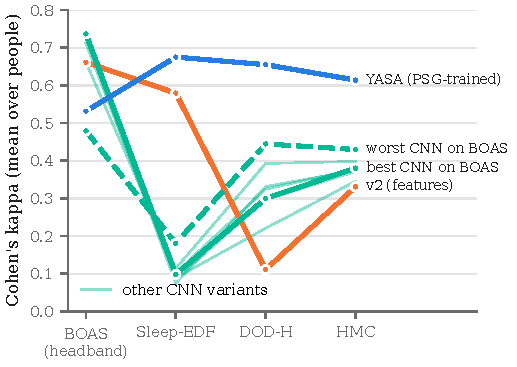
\includegraphics[width=\linewidth]{figures/fig1_ranking.pdf}
\caption{Kappa on held-out BOAS people and on three external datasets. Each line is one frozen model.
The order on the headband does not carry over.}
\label{fig:ranking}
\end{figure}

\begin{table*}[t]
\centering\small
\caption{Main benchmark, whole-recording window. Mean over people, with 95\% bootstrap intervals.
BOAS: 20 people; Sleep-EDF: 20; DOD-H: 25; HMC: 25.}
\label{tab:bench}
% Generated by paper/make_numbers.py. Do not edit by hand.
\begin{tabular}{llcccc}
\toprule
Dataset & Model & Kappa & Macro-F1 & Wake F1 & Sleep-time error (min) \\
\midrule
BOAS & YASA & \val{boas}{yasa}{kappa} {\scriptsize[\val{boas}{yasa}{kappa_lo}, \val{boas}{yasa}{kappa_hi}]} & \val{boas}{yasa}{macro_f1} {\scriptsize[\val{boas}{yasa}{macro_f1_lo}, \val{boas}{yasa}{macro_f1_hi}]} & \val{boas}{yasa}{wake_f1} {\scriptsize[\val{boas}{yasa}{wake_f1_lo}, \val{boas}{yasa}{wake_f1_hi}]} & \val{boas}{yasa}{tst_error_minutes} {\scriptsize[\val{boas}{yasa}{tst_error_minutes_lo}, \val{boas}{yasa}{tst_error_minutes_hi}]} \\
 & v2 & \val{boas}{v2}{kappa} {\scriptsize[\val{boas}{v2}{kappa_lo}, \val{boas}{v2}{kappa_hi}]} & \val{boas}{v2}{macro_f1} {\scriptsize[\val{boas}{v2}{macro_f1_lo}, \val{boas}{v2}{macro_f1_hi}]} & \val{boas}{v2}{wake_f1} {\scriptsize[\val{boas}{v2}{wake_f1_lo}, \val{boas}{v2}{wake_f1_hi}]} & \val{boas}{v2}{tst_error_minutes} {\scriptsize[\val{boas}{v2}{tst_error_minutes_lo}, \val{boas}{v2}{tst_error_minutes_hi}]} \\
 & CNN & \val{boas}{cnn}{kappa} {\scriptsize[\val{boas}{cnn}{kappa_lo}, \val{boas}{cnn}{kappa_hi}]} & \val{boas}{cnn}{macro_f1} {\scriptsize[\val{boas}{cnn}{macro_f1_lo}, \val{boas}{cnn}{macro_f1_hi}]} & \val{boas}{cnn}{wake_f1} {\scriptsize[\val{boas}{cnn}{wake_f1_lo}, \val{boas}{cnn}{wake_f1_hi}]} & \val{boas}{cnn}{tst_error_minutes} {\scriptsize[\val{boas}{cnn}{tst_error_minutes_lo}, \val{boas}{cnn}{tst_error_minutes_hi}]} \\
 & CNN, balanced & \val{boas}{cnn_balanced}{kappa} {\scriptsize[\val{boas}{cnn_balanced}{kappa_lo}, \val{boas}{cnn_balanced}{kappa_hi}]} & \val{boas}{cnn_balanced}{macro_f1} {\scriptsize[\val{boas}{cnn_balanced}{macro_f1_lo}, \val{boas}{cnn_balanced}{macro_f1_hi}]} & \val{boas}{cnn_balanced}{wake_f1} {\scriptsize[\val{boas}{cnn_balanced}{wake_f1_lo}, \val{boas}{cnn_balanced}{wake_f1_hi}]} & \val{boas}{cnn_balanced}{tst_error_minutes} {\scriptsize[\val{boas}{cnn_balanced}{tst_error_minutes_lo}, \val{boas}{cnn_balanced}{tst_error_minutes_hi}]} \\
\midrule
Sleep-EDF & YASA & \val{sleep_edf}{yasa}{kappa} {\scriptsize[\val{sleep_edf}{yasa}{kappa_lo}, \val{sleep_edf}{yasa}{kappa_hi}]} & \val{sleep_edf}{yasa}{macro_f1} {\scriptsize[\val{sleep_edf}{yasa}{macro_f1_lo}, \val{sleep_edf}{yasa}{macro_f1_hi}]} & \val{sleep_edf}{yasa}{wake_f1} {\scriptsize[\val{sleep_edf}{yasa}{wake_f1_lo}, \val{sleep_edf}{yasa}{wake_f1_hi}]} & \val{sleep_edf}{yasa}{tst_error_minutes} {\scriptsize[\val{sleep_edf}{yasa}{tst_error_minutes_lo}, \val{sleep_edf}{yasa}{tst_error_minutes_hi}]} \\
 & v2 & \val{sleep_edf}{v2}{kappa} {\scriptsize[\val{sleep_edf}{v2}{kappa_lo}, \val{sleep_edf}{v2}{kappa_hi}]} & \val{sleep_edf}{v2}{macro_f1} {\scriptsize[\val{sleep_edf}{v2}{macro_f1_lo}, \val{sleep_edf}{v2}{macro_f1_hi}]} & \val{sleep_edf}{v2}{wake_f1} {\scriptsize[\val{sleep_edf}{v2}{wake_f1_lo}, \val{sleep_edf}{v2}{wake_f1_hi}]} & \val{sleep_edf}{v2}{tst_error_minutes} {\scriptsize[\val{sleep_edf}{v2}{tst_error_minutes_lo}, \val{sleep_edf}{v2}{tst_error_minutes_hi}]} \\
 & CNN & \val{sleep_edf}{cnn}{kappa} {\scriptsize[\val{sleep_edf}{cnn}{kappa_lo}, \val{sleep_edf}{cnn}{kappa_hi}]} & \val{sleep_edf}{cnn}{macro_f1} {\scriptsize[\val{sleep_edf}{cnn}{macro_f1_lo}, \val{sleep_edf}{cnn}{macro_f1_hi}]} & \val{sleep_edf}{cnn}{wake_f1} {\scriptsize[\val{sleep_edf}{cnn}{wake_f1_lo}, \val{sleep_edf}{cnn}{wake_f1_hi}]} & \val{sleep_edf}{cnn}{tst_error_minutes} {\scriptsize[\val{sleep_edf}{cnn}{tst_error_minutes_lo}, \val{sleep_edf}{cnn}{tst_error_minutes_hi}]} \\
 & CNN, balanced & \val{sleep_edf}{cnn_balanced}{kappa} {\scriptsize[\val{sleep_edf}{cnn_balanced}{kappa_lo}, \val{sleep_edf}{cnn_balanced}{kappa_hi}]} & \val{sleep_edf}{cnn_balanced}{macro_f1} {\scriptsize[\val{sleep_edf}{cnn_balanced}{macro_f1_lo}, \val{sleep_edf}{cnn_balanced}{macro_f1_hi}]} & \val{sleep_edf}{cnn_balanced}{wake_f1} {\scriptsize[\val{sleep_edf}{cnn_balanced}{wake_f1_lo}, \val{sleep_edf}{cnn_balanced}{wake_f1_hi}]} & \val{sleep_edf}{cnn_balanced}{tst_error_minutes} {\scriptsize[\val{sleep_edf}{cnn_balanced}{tst_error_minutes_lo}, \val{sleep_edf}{cnn_balanced}{tst_error_minutes_hi}]} \\
\midrule
DOD-H & YASA & \val{dodh}{yasa}{kappa} {\scriptsize[\val{dodh}{yasa}{kappa_lo}, \val{dodh}{yasa}{kappa_hi}]} & \val{dodh}{yasa}{macro_f1} {\scriptsize[\val{dodh}{yasa}{macro_f1_lo}, \val{dodh}{yasa}{macro_f1_hi}]} & \val{dodh}{yasa}{wake_f1} {\scriptsize[\val{dodh}{yasa}{wake_f1_lo}, \val{dodh}{yasa}{wake_f1_hi}]} & \val{dodh}{yasa}{tst_error_minutes} {\scriptsize[\val{dodh}{yasa}{tst_error_minutes_lo}, \val{dodh}{yasa}{tst_error_minutes_hi}]} \\
 & v2 & \val{dodh}{v2}{kappa} {\scriptsize[\val{dodh}{v2}{kappa_lo}, \val{dodh}{v2}{kappa_hi}]} & \val{dodh}{v2}{macro_f1} {\scriptsize[\val{dodh}{v2}{macro_f1_lo}, \val{dodh}{v2}{macro_f1_hi}]} & \val{dodh}{v2}{wake_f1} {\scriptsize[\val{dodh}{v2}{wake_f1_lo}, \val{dodh}{v2}{wake_f1_hi}]} & \val{dodh}{v2}{tst_error_minutes} {\scriptsize[\val{dodh}{v2}{tst_error_minutes_lo}, \val{dodh}{v2}{tst_error_minutes_hi}]} \\
 & CNN & \val{dodh}{cnn}{kappa} {\scriptsize[\val{dodh}{cnn}{kappa_lo}, \val{dodh}{cnn}{kappa_hi}]} & \val{dodh}{cnn}{macro_f1} {\scriptsize[\val{dodh}{cnn}{macro_f1_lo}, \val{dodh}{cnn}{macro_f1_hi}]} & \val{dodh}{cnn}{wake_f1} {\scriptsize[\val{dodh}{cnn}{wake_f1_lo}, \val{dodh}{cnn}{wake_f1_hi}]} & \val{dodh}{cnn}{tst_error_minutes} {\scriptsize[\val{dodh}{cnn}{tst_error_minutes_lo}, \val{dodh}{cnn}{tst_error_minutes_hi}]} \\
 & CNN, balanced & \val{dodh}{cnn_balanced}{kappa} {\scriptsize[\val{dodh}{cnn_balanced}{kappa_lo}, \val{dodh}{cnn_balanced}{kappa_hi}]} & \val{dodh}{cnn_balanced}{macro_f1} {\scriptsize[\val{dodh}{cnn_balanced}{macro_f1_lo}, \val{dodh}{cnn_balanced}{macro_f1_hi}]} & \val{dodh}{cnn_balanced}{wake_f1} {\scriptsize[\val{dodh}{cnn_balanced}{wake_f1_lo}, \val{dodh}{cnn_balanced}{wake_f1_hi}]} & \val{dodh}{cnn_balanced}{tst_error_minutes} {\scriptsize[\val{dodh}{cnn_balanced}{tst_error_minutes_lo}, \val{dodh}{cnn_balanced}{tst_error_minutes_hi}]} \\
\midrule
HMC & YASA & \val{hmc}{yasa}{kappa} {\scriptsize[\val{hmc}{yasa}{kappa_lo}, \val{hmc}{yasa}{kappa_hi}]} & \val{hmc}{yasa}{macro_f1} {\scriptsize[\val{hmc}{yasa}{macro_f1_lo}, \val{hmc}{yasa}{macro_f1_hi}]} & \val{hmc}{yasa}{wake_f1} {\scriptsize[\val{hmc}{yasa}{wake_f1_lo}, \val{hmc}{yasa}{wake_f1_hi}]} & \val{hmc}{yasa}{tst_error_minutes} {\scriptsize[\val{hmc}{yasa}{tst_error_minutes_lo}, \val{hmc}{yasa}{tst_error_minutes_hi}]} \\
 & v2 & \val{hmc}{v2}{kappa} {\scriptsize[\val{hmc}{v2}{kappa_lo}, \val{hmc}{v2}{kappa_hi}]} & \val{hmc}{v2}{macro_f1} {\scriptsize[\val{hmc}{v2}{macro_f1_lo}, \val{hmc}{v2}{macro_f1_hi}]} & \val{hmc}{v2}{wake_f1} {\scriptsize[\val{hmc}{v2}{wake_f1_lo}, \val{hmc}{v2}{wake_f1_hi}]} & \val{hmc}{v2}{tst_error_minutes} {\scriptsize[\val{hmc}{v2}{tst_error_minutes_lo}, \val{hmc}{v2}{tst_error_minutes_hi}]} \\
 & CNN & \val{hmc}{cnn}{kappa} {\scriptsize[\val{hmc}{cnn}{kappa_lo}, \val{hmc}{cnn}{kappa_hi}]} & \val{hmc}{cnn}{macro_f1} {\scriptsize[\val{hmc}{cnn}{macro_f1_lo}, \val{hmc}{cnn}{macro_f1_hi}]} & \val{hmc}{cnn}{wake_f1} {\scriptsize[\val{hmc}{cnn}{wake_f1_lo}, \val{hmc}{cnn}{wake_f1_hi}]} & \val{hmc}{cnn}{tst_error_minutes} {\scriptsize[\val{hmc}{cnn}{tst_error_minutes_lo}, \val{hmc}{cnn}{tst_error_minutes_hi}]} \\
 & CNN, balanced & \val{hmc}{cnn_balanced}{kappa} {\scriptsize[\val{hmc}{cnn_balanced}{kappa_lo}, \val{hmc}{cnn_balanced}{kappa_hi}]} & \val{hmc}{cnn_balanced}{macro_f1} {\scriptsize[\val{hmc}{cnn_balanced}{macro_f1_lo}, \val{hmc}{cnn_balanced}{macro_f1_hi}]} & \val{hmc}{cnn_balanced}{wake_f1} {\scriptsize[\val{hmc}{cnn_balanced}{wake_f1_lo}, \val{hmc}{cnn_balanced}{wake_f1_hi}]} & \val{hmc}{cnn_balanced}{tst_error_minutes} {\scriptsize[\val{hmc}{cnn_balanced}{tst_error_minutes_lo}, \val{hmc}{cnn_balanced}{tst_error_minutes_hi}]} \\
\bottomrule
\end{tabular}

\end{table*}

\subsection{The pre-registered external test}

\textbf{H1, amplitude.} DOD-H's signals are about four times smaller than the headband's (estimated
gain \val{gain}{dodh}{q75}). Uncalibrated v2 fell apart there (kappa \val{dodh}{v2}{kappa}), and the
correction won back a large part of it: macro-F1 $+0.161$ [0.119, 0.202], kappa $+0.207$ [0.145, 0.273],
sleep-time error $-11.3$ minutes [$-19.1$, $-2.3$]. H1 and H1b were supported, and they are the only
two tests that survive Holm correction. On HMC the estimated gain was a modest \val{gain}{hmc}{q75},
and applying it made v2 worse: macro-F1 $-0.088$ [$-0.127$, $-0.049$], sleep-time error $+81.7$ minutes
[49.8, 117.5]. Both were contradicted. A look at the errors afterwards shows what happened. Scaling the
signal up pushed REM, whose EEG is the closest to wake, over the line: the share of reference REM
labelled wake went from 11\% to 43\%. The gain statistic responds to montage, population and the
amount of wake as well as to amplitude, so it overshoots when the real mismatch is small.

\textbf{H2, wake.} The plain CNN's wake recall was 0.503 [0.420, 0.586] on DOD-H and 0.638
[0.561, 0.710] on HMC. Both fall between the pre-registered thresholds, so H2 is mixed on both. On
Sleep-EDF the same model found 0.13 of wake. The near-total loss of wake there does not repeat on
night recordings, though the CNN still misses between a third and a half of it.

\textbf{Headline.} The pre-registration held two headlines written in advance. The data picked the
second: choosing by in-domain score did not find the models that travel, and amplitude correction
explained part of the drop on only one of the two new datasets.

\subsection{Why the CNNs lose wake}

Several explanations fell away on Sleep-EDF. Changing the normalisation window or rescaling the input
moved the CNN's macro-F1 by no more than 0.001, as the instance-normalisation argument predicted.
Cropping to a label-free night window hardly helped; only an oracle window built from the labels
removed the sleep-time error. Feeding it Pz-Oz instead of Fpz-Cz raised wake recall from 0.13 to 0.37,
still far below the 0.87 it reaches on the headband. Rebuilding the input files from the original
recordings reproduced them bit for bit, so it is not a preprocessing bug.

The wake spectrum points somewhere else. Headband wake carries about twice the 16--30\,Hz share of
Sleep-EDF wake (0.071 against 0.038), which is what forehead muscle activity would do. Taking 16--30\,Hz
out of the frozen CNN's input (Figure~\ref{fig:mech}b) lowers the wake probability of wake epochs on
every dataset, by two to four times more than it lowers that of sleep epochs. That makes it a genuine
wake cue, and one the network uses on every device, not only on the headband. Taking out 0.5--4\,Hz has
a bigger effect, but it raises the wake probability of sleep epochs just as much, so that band is the
network's general sign of sleep rather than anything specific to wake.

I then tested, under a pre-registered addendum, whether removing that reliance helps. A CNN trained
with 16--30\,Hz dropped at random raised wake recall on all three external datasets on the original
seed, and the effect survived Holm correction. A replicate-seed check, added after that result and
logged as a departure from the plan, took it apart (Figure~\ref{fig:mech}a). The retrained models had
used 10 training passes while the frozen CNN had used 25, a mismatch I found later and logged, so the
check compares each model with a 10-pass plain CNN of the same seed. Across five seeds that plain CNN's
headband kappa stayed between \val{seeds}{boas_kappa}{min} and \val{seeds}{boas_kappa}{max}, while its
wake recall ranged from \val{seeds}{sleep_edf_wake_recall}{min} to \val{seeds}{sleep_edf_wake_recall}{max}
on Sleep-EDF, \val{seeds}{dodh_wake_recall}{min} to \val{seeds}{dodh_wake_recall}{max} on DOD-H and
\val{seeds}{hmc_wake_recall}{min} to \val{seeds}{hmc_wake_recall}{max} on HMC. Training length was not
the cause: at the original seed, 10 and 25 passes gave 0.10 and 0.13 on Sleep-EDF. Four of the nine
matched-seed comparisons for the dropout model were at or below zero, and pooled over seeds it helped a
little on Sleep-EDF and DOD-H and hurt on HMC. Any single-seed CNN comparison in this work, the H2
verdict on HMC included, has to be read against that spread.

\begin{figure*}[t]
\centering
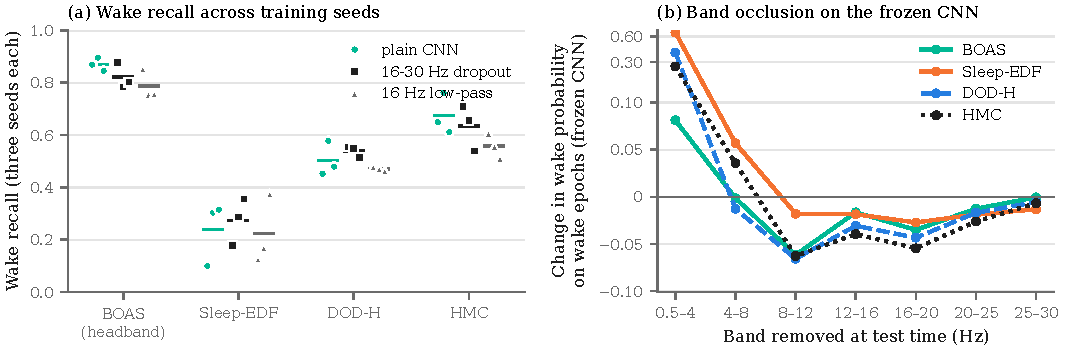
\includegraphics[width=\linewidth]{figures/fig2_mechanism.pdf}
\caption{(a) Wake recall of three CNN recipes, one dot per training seed (five for the plain CNN, three
for the others); bars are means. The spread across seeds is as wide as the gap between recipes.
(b) Change in the frozen CNN's wake probability on reference-wake epochs when one band is removed at
test time (symmetric log scale).}
\label{fig:mech}
\end{figure*}

\subsection{Recording length and the sleep-time error}

On Sleep-EDF, v2 overestimated sleep by 236 minutes on average, because most of each recording is
daytime wake and it labels part of that as sleep (Figure~\ref{fig:failure}). A detector that needs no
labels and keeps the longest smoothed run of sleep, with its two settings chosen on 56 development
recordings, brought v2's error down to 158 minutes and YASA's from 110 to 41. On night recordings it
made things slightly worse. Used only on recordings longer than 14.4 hours, a cut-off taken from the
lengths of training and development recordings, it keeps the gain on Sleep-EDF and leaves every night
recording untouched. No test recording comes near the cut-off, so the rule is safe here but has not
really been tested.

\begin{figure*}[t]
\centering
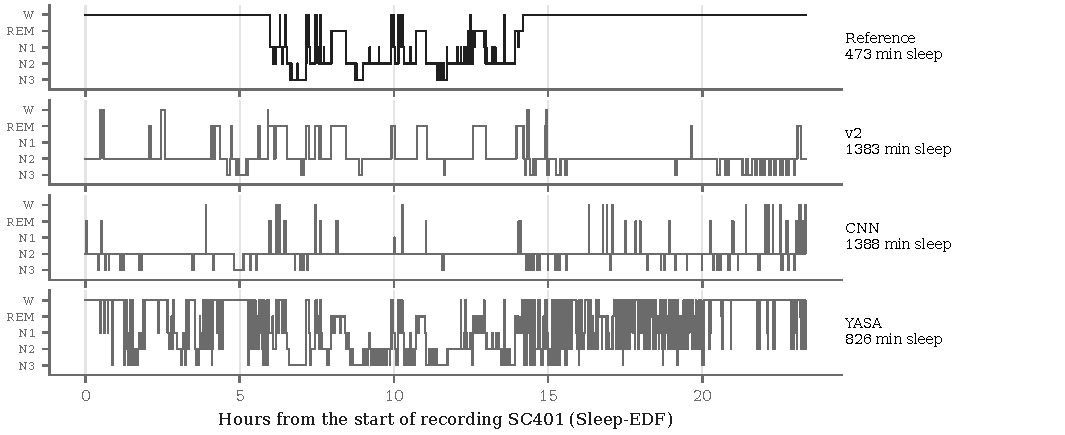
\includegraphics[width=\linewidth]{figures/fig3_failure_case.pdf}
\caption{A Sleep-EDF recording whose reference has 473 minutes of sleep in 23 hours. v2 and the CNN
label most of the day N2. YASA follows the night but also scores scattered sleep in the daytime.}
\label{fig:failure}
\end{figure*}

\subsection{Can confidence protect a claim?}

Figure~\ref{fig:rc} shows risk--coverage curves, with epochs ranked by the model's top probability. On
BOAS the epochs both models are sure of are mostly right. Off the headband this breaks. On Sleep-EDF
the CNN's most confident epochs are mostly wrong (area under the curve 0.64), and on HMC the epochs v2
is most sure of are wrong more often than its epochs overall. A gate at the level of the whole
recording, which withholds the sleep-time figure when the estimated gain is far from one, did better
where the mismatch was real. It blocked 4 of 12 large errors on Sleep-EDF without withholding a good
figure, and flagged 24 of 25 DOD-H recordings as out of range. On BOAS it held back four good figures to
stop one bad one. A useful gate needs more than one amplitude statistic.

\begin{figure*}[t]
\centering
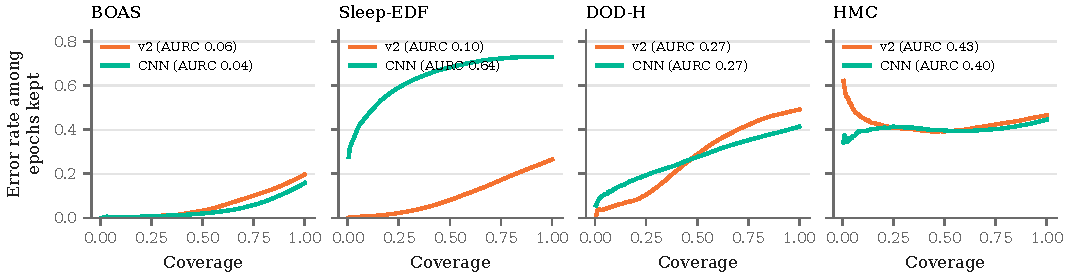
\includegraphics[width=\linewidth]{figures/fig4_risk_coverage.pdf}
\caption{Risk--coverage curves: the error rate among the epochs kept, keeping epochs in order of the
model's own confidence. Lower is better.}
\label{fig:rc}
\end{figure*}

\subsection{The gap to the vendor's scorer}

BOAS ships with the device maker's own stager. On the epochs it labels, it reaches kappa
\val{bb}{vendor_covered}{bitbrain} on the test people, against \val{bb}{vendor_covered}{cnn_ensemble}
for an ensemble of seven CNNs. In one exploratory attempt I averaged the ensemble's probabilities with
v2's, with the weight (\val{bb}{w}{v2} for v2) chosen on six selection people only. On the test people
this reached \val{bb}{vendor_covered}{fusion}, and what is left of the gap to the vendor,
$\val{bb}{paired}{fusion_minus_bitbrain_vendor_covered}$ [$\val{bb}{paired}{fusion_minus_bitbrain_vendor_covered_lo}$,
$\val{bb}{paired}{fusion_minus_bitbrain_vendor_covered_hi}$], can no longer be told apart from zero.
The test people had been looked at before, so all this shows is that the two model families make
different mistakes on the headband.

\section{Discussion}

The practical lesson is about selection. If a model is going to a new device, choose it on validation
data that looks like that device, not only on held-out people from the old one. Here the in-domain
score was close to useless for that choice. The most useful single fact was one the in-domain score
could not have shown: YASA, trained on many clinical recordings, held up under the change of device,
and none of the models trained on one headband did.

The two families broke in different ways. v2 depends on absolute amplitude, so a gross gain mismatch
wrecks it and a label-free correction repairs much of the damage; a small mismatch is better left
alone. The CNNs are built to ignore amplitude and fail on wake instead, partly because they learned a
high-frequency wake cue that clinical frontal channels carry less of. Neither failure showed up on
held-out headband people.

The seed result is the one I would most like someone else to check. Five networks that are
indistinguishable on the headband differ by more than a factor of three in how much wake they find on
Sleep-EDF.
That is underspecification in the sense of D'Amour et al.\ \cite{damour2022}, and it means that a
single-seed comparison of two architectures or augmentations under device shift can say very little,
however carefully its in-domain score was measured.

\textbf{Future work.} Engineering first: a shift check that withholds the sleep-time figure when a
recording falls outside the training conditions, and a viewer that shows when it does. On the research
side: train the sleep-window detector on data with real daytime wake, replace the single gain statistic
with a detector that uses several features, repeat the ranking test with more model families and more
seeds, and validate on paired headband and PSG nights recorded for the purpose. Further out, the daytime
half of the original idea, attention during a focus task, needs its own consented recordings and ethics
approval.

\section{Limitations}

Sleep-EDF was looked at during development, so only DOD-H and HMC are clean tests, with 25 people each.
All the training data and two of the three external datasets come from healthy adults; HMC is a
clinical sample, but a small one. Rank correlations over this many models are imprecise, as their
intervals show. The frozen CNN numbers come from one training seed, and the seed check shows how much
that matters. DOD-H's signals are band-limited compared with the others, which I noted before scoring
but which still muddies the H2 reading there. The H2 thresholds I chose turned out to sit either side of
the values observed, which made a mixed verdict likely. Nothing here supports clinical use.

\section*{Data and code availability}
The repository linked above holds all code, the frozen models, every saved prediction and metric file,
the pre-registration with its amendments and deviations, and the scripts that produce every figure and
number in this paper. Raw recordings are downloaded from their original sources by scripts in the
repository. A Zenodo archive accompanies this version.

\section*{Acknowledgements}
The project started at the Oxford NeuroTech Hackathon in November 2026. The research reported here was
done afterwards by the author alone.

\small
\bibliographystyle{unsrtnat}
\bibliography{refs}

\onecolumn
\appendix
\section{Appendix}

\subsection{All headband models}
Full metrics for every model and dataset, including the CNN variants left out of
Table~\ref{tab:bench}, are in \texttt{results/paper/benchmark.json}. The script that writes it
recomputes every value from the saved predictions and checks 108 of them against the metric files
written at evaluation time. The wider ranking test and the five-seed spread are in
\texttt{results/paper/ranking\_extended.json}.

\subsection{Pre-registration verdicts}
\begin{center}\small
\begin{tabular}{lll}
\toprule
Test & DOD-H (25) & HMC (25) \\
\midrule
H1, macro-F1, v2 + gain vs v2 & supported: $+0.161$ [0.119, 0.202] & contradicted: $-0.088$ [$-0.127$, $-0.049$] \\
H1b, sleep-time error (min) & supported: $-11.3$ [$-19.1$, $-2.3$] & contradicted: $+81.7$ [49.8, 117.5] \\
H1b, kappa & supported: $+0.207$ [0.145, 0.273] & contradicted: $-0.088$ [$-0.135$, $-0.044$] \\
H2, CNN wake recall & mixed: 0.503 (v2 0.142) & mixed: 0.638 (v2 0.760) \\
Family gap, macro-F1 & mixed: $-0.149$ & closes: $-0.034$ [$-0.075$, 0.005] \\
\bottomrule
\end{tabular}
\end{center}

\subsection{Checks added after the pre-registered result}
These were logged as addenda before they were run. Holm correction across the six wake tests of the
retrained CNNs: on the original seed all three dropout results stayed significant (adjusted $p$ =
0.001, 0.019 and 0.002). Replicate seeds: see the Results. Band occlusion: the prediction that the
16--30\,Hz bands would matter more on BOAS than on the external datasets failed; the summed drop in
wake probability was 0.048 on BOAS against 0.059, 0.066 and 0.088 elsewhere. Calibration: the plain
CNN's expected calibration error was 0.053 on BOAS and 0.419 on Sleep-EDF.

\subsection{Labelling scheme}
BOAS has little N3: 3.6\% of scored epochs, against 14.0\% on DOD-H and 20.5\% on HMC. Every
headband-trained model under-calls N3 everywhere, BOAS included, where v2 sends 41\% of reference N3 to
N2. The shortfall comes from the training labels.

\subsection{The drug-delivery track}
The hackathon project had a second, separate track: predicting brain exposure from blood exposure and
formulation, using the supporting data of Yousfan et al.\ \cite{yousfan2024} (402 rows, held out by
source study). Measured blood exposure carried nearly all the signal. Formulation descriptors did not
transfer across studies, and adding them made predictions worse. A leakage audit found two measurements
reported under two study titles each; once those were merged, the best model could no longer be told
apart from a route-specific brain/blood ratio (difference interval $-0.097$ to $+0.015$ on the log
scale). For this paper the model and the audit were rerun from the original workbook (same checksum as
the event run), and every stored value came out the same. The workbook is licensed for non-commercial
use and is not redistributed; the outputs are in \texttt{neurorelease/exposure\_model/out/}.

\subsection{Author contributions}
B.B.\ designed the study, wrote the pre-registration, built and evaluated the models, analysed the
results and wrote the paper.

\end{document}
